\documentclass[a4paper,singleside,12pt]{report} % Uncomment this for single side pdf.
%\documentclass[a4paper,twoside,12pt]{report} % Uncomment this for printing.

\usepackage{ai_bo_thesis}
\usepackage[english]{babel}
\usepackage[T1]{fontenc}
\usepackage{amsmath}   % For equations
\usepackage{lmodern}
\usepackage{hyperref}  % Fixes \href errors
\usepackage{xurl}      % Allows line breaks in URLs
\usepackage{booktabs}  % Fixes \toprule, \midrule, \bottomrule errors
\usepackage{multirow}
\usepackage{graphicx}
\usepackage{caption}
\usepackage{subcaption}
\setlength{\headheight}{14.5pt}  % Fixes fancyhdr warning

\usepackage{csquotes} % Recommended for proper quotation handling
\usepackage[backend=biber, style=numeric, sorting=nty, firstinits=true]{biblatex}
\addbibresource{biblio.bib}

\setmainfont{Times New Roman}
\begin{document}

\title{Hardware Dimensioning for Environmental Sustainability: benchmark of AI algorithms and environmental impact}
\topic{Intelligent Systems}
\candidate{Enrico Morselli}
\supervisor{Prof.~Andrea Borghesi}
\cosupervisor{& Prof.~Allegra De Filippo} % One co-supervisor.
%	\cosupervisors{& Dott.~Ing.~Luigi Bianchi\\& Dott~Avv.~Lucia Rossi} % More than one co-supervisor.
\academicyear{2024-2025}
\session{5th}

\frontispiece 
\dedication{Dedicated to my Grandma}
\toc
\figstoc
\tablestoc
\begintext

\chapter{Introduction}

\section{Background and Rationale}

\section{Introduction}

In recent years, we have witnessed a dramatic improvement in the performance of Artificial Intelligence (AI) technologies. 
While AI still falls short of human ability in some complex cognitive tasks, as of 2023, it has surpassed human capabilities 
in various domains, including image classification, basic reading comprehension, visual reasoning, and natural language inference 
\cite{AIIndexReport}. Moreover, Generative AI has achieved astonishing results in areas such as image and video generation, further 
demonstrating the rapid advancements in the field \cite{AIIndexReport}. 

These remarkable gains in AI performance have been primarily driven by the large-scale expansion of model sizes and computational 
resources (often referred to as "compute") dedicated to training state-of-the-art AI models. Research indicates that, for frontier 
AI models—those that ranked among the top 10 in terms of training compute at the time of their release—the amount of compute used
for training has been increasing at an exponential rate, growing by a factor of 4-5x per year since 2010 \cite{epoch2024compute}. 

However, this surge in compute requirements has led to a corresponding increase in energy consumption, which, in turn, has 
amplified the environmental impact of AI due to $\mathsf{CO_2}$ emissions. For instance, the training of Meta AI's LLaMA models 
was estimated to take approximately five months on a cluster of $2048$ $\mathsf{A}100$ $80\mathsf{GB}$ GPUs, consuming a total 
of $2,638$ $\mathsf{MWh}$ of energy and producing approximately $1,015$ $\mathsf{tCO_2eq}$ in emissions \cite{touvron2023llama}. 
Given the growing adoption of AI technologies, the rapid increase in model size and complexity, and the escalating energy demands 
of AI applications, the carbon footprint of AI has become an increasingly pressing concern, particularly in the context of the 
ongoing climate emergency.

In this work, we explore a novel approach to addressing the sustainability challenges of AI by extending the HADA (HArdware 
Dimensioning for AI Algorithms) framework. HADA is a framework that leverages Machine Learning (ML) to learn the relationship 
between an algorithm's configuration and its performance metrics—such as total runtime, solution cost, and memory usage—and then 
employs optimization techniques to identify the optimal hardware architecture and configuration that meet predefined performance 
and budget constraints. This process, known as Hardware Dimensioning, has been studied as a means to efficiently allocate 
computational resources while maintaining performance requirements \cite{DEFILIPPO2022109199}. 

Our contribution extends HADA by incorporating energy consumption and carbon emissions as additional performance metrics. 
By doing so, we aim to identify the best combination of algorithm and hardware configuration that minimizes the environmental 
impact of computation. To validate our approach, we will conduct experiments on small-scale algorithms that can be executed in 
a timely manner on local machines and high-performance computing (HPC) clusters. Ultimately, we seek to demonstrate how AI 
workloads can be optimized not only for efficiency and cost but also for sustainability, thus contributing to the broader goal 
of reducing AI's carbon footprint.

% TODO: expand the "Rest of the work" section

The rest of the work is structured as follows:
\begin{itemize}
    \item \textbf{Chapter 2} Reviews the environmental impact of AI, with case studies on the carbon footprint of training large models like GPT-3. It then discusses the concept of "Green AI" vs. "Red AI"—balancing accuracy with sustainability, and covers existing tools for tracking AI energy consumption and carbon emissions, such as ML CO2 Impact and CodeCarbon.
    \item \textbf{Chapter 3} Introduces the Empirical Model Learning (EML) approach, on which HADA is based on. Describes HADA's three-phase workflow: data collection, surrogate model training, and optimization. It then defines the methodology for tracking carbon emissions and integrates it into HADA’s hardware dimensioning process.
    \item \textbf{Chapter 4} Presents benchmarking results for different AI algorithms, and analyzes energy consumption and CO2 emissions across different hardware platforms.
    \item \textbf{Chapter 5} Introduces the HADA Web Application, which provides a user-friendly interface for optimizing AI workloads. Describes how users can select algorithms, define optimization constraints, and choose geographic locations to assess energy efficiency.
    \item \textbf{Chapter 6} Summarizes key findings, emphasizing the importance of sustainability in AI computation and concludes the work.
\end{itemize}

\chapter{Related Works}

\section{Sustainability in AI}

The environmental impact of training large AI models has been underscored by recent empirical assessments. Strubell et al. (2019)
quantified the $\mathsf{CO_2}$ emissions of several Natural Language Processing (NLP) models and discovered that training a large
transformer with extensive hyperparameter tuning, including neural architecture search, emitted approximately 626,000 pounds 
(around 284 metric tons) of $\mathsf{CO_2}$—comparable to the lifetime emissions of five cars \cite{strubell2019energy}. 
Another study found out that GPT-3 released 552 metric tons of $\mathsf{CO_2}$ into the atmosphere during training, the 
equivalent of 123 gasoline-powered passenger vehicles driven for one year \cite{patterson2021carbon}. These findings highlight that 
improvements in AI accuracy often come at a significant energy and carbon cost.

In response to these concerns, researchers have begun systematically reporting energy usage and the resulting $\mathsf{CO_2}$ 
emissions associated with model training to raise awareness \cite{dodge2022carbon, patterson2021carbon}. Transparent reporting 
is essential for understanding and ultimately mitigating AI's climate impacts. For instance, Henderson et al. (2020) introduced 
a framework for tracking real-time energy consumption and carbon emissions during Machine Learning (ML) experiments, encouraging 
researchers to include these metrics in their publications \cite{henderson2020carbon}.

Broader studies have examined AI's total energy and environmental footprint across the industry. Gupta et al. (2021) analyzed 
the end-to-end footprint of computing and found that while operational emissions (from running hardware) have been partly curbed 
by efficiency improvements, the overall carbon footprint of computing continues to grow due to increased scale. Notably, they 
showed that for modern data centers and mobile devices, manufacturing and infrastructure (embodied carbon) now account for the 
majority of emissions. As data centers adopt cleaner power, the emissions embedded in hardware supply chains—such as chip 
fabrication and server manufacturing—become a dominant concern. \cite{gupta2020carbon}

Similarly, Wu et al. (2022) conducted a comprehensive study of AI at a large technology company (Meta/Facebook), examining the 
entire AI model lifecycle—from data processing and training to inference and hardware lifecycle. They reported super-linear 
growth in AI workloads and infrastructure; for instance, daily inference operations doubled over a recent three-year span, 
necessitating a 2.5x expansion in server capacity. Crucially, Wu et al. also highlighted that embodied carbon is an increasing 
fraction of AI's total footprint, echoing that improvements in hardware efficiency alone cannot eliminate AI's impact. Their 
analysis argues for looking beyond training alone—considering data center construction, supply chains, and the frequency of 
model retraining—to truly grasp AI's environmental impact. \cite{wu2021sustainableai}

A recurring theme in these studies is the diminishing return on energy investment for AI model improvements. As models become 
larger and more complex, incremental accuracy gains often require disproportionately more compute power, and thus energy. 
Schwartz et al. (2020) termed this phenomenon "Red AI," where researchers prioritize accuracy regardless of computational cost, 
and noted this trend is unsustainable both environmentally and economically \cite{GreenAI}. Thompson et al. (2021) similarly 
observed that progress in benchmarks was accompanied by exponentially increasing computing costs, warning of diminishing returns 
and calling the situation unsustainable. \cite{thompson2021deeplearning}

Another challenge is equitable access: massive energy requirements make cutting-edge AI research expensive, potentially 
concentrating it in wealthy institutions and regions with robust infrastructure. This raises concerns that AI's growing energy 
demands not only harm the planet but also exacerbate inequalities in who can afford to conduct top-tier research. These concerns 
have prompted calls for a paradigm shift toward "Green AI," where efficiency and sustainability are treated as primary goals in 
model development.

In summary, the environmental sustainability of AI has become a critical area of concern. As the field advances, it is 
imperative to balance the pursuit of performance improvements with the need to minimize energy consumption and carbon emissions. 
This balance is essential not only for mitigating climate change but also for ensuring equitable access to AI research and 
development.

\section{Tools for Tracking Carbon Emissions}

The increasing awareness of AI’s carbon footprint has motivated the development of dedicated tools and methodologies for monitoring 
the environmental impact of AI workloads. A number of open-source tools and frameworks have been introduced to help practitioners 
measure the energy consumption and $\mathsf{CO_2}$ emissions of their code, enabling more informed decisions about sustainability 
in AI research and deployment.

One of the early tools for estimating emissions from model training was \textbf{ML CO2 Impact} (Machine Learning 
Emissions Calculator), introduced by Lacoste et al. (2019) \cite{lacoste2019quantifying}. This web-based calculator allows users 
to input key information about their training runs—such as hardware type (CPU/GPU), runtime, cloud provider, and location—and 
computes the corresponding energy consumption and carbon emissions. The tool relies on known power draw profiles of hardware 
components and regional carbon intensity factors to generate estimates. According to Bannour et al. (2021) 
\cite{bannour-etal-2021-evaluating}, the latest iteration of this tool has evolved under the umbrella of the \textbf{CodeCarbon} 
initiative, integrating its functionality into the open-source CodeCarbon package.

\textbf{CodeCarbon} \cite{courty2024codecarbon}, which is the tool we employ in this work to enhance HADA, is an open-source 
Python package designed to track the carbon footprint of computing projects. It integrates seamlessly into ML workflows, 
logging resource usage (CPU, GPU, and other components) and estimating the $\mathsf{CO_2}$ emissions produced by the workload. 
A key feature of CodeCarbon is its ability to account for the geographic location of the computation—leveraging region-specific 
electricity carbon intensity data to provide location-dependent emission estimates. \textbf{Carbon Intensity} refers to the 
amount of $\mathsf{CO_2}$ emitted per unit of electricity generated, typically measured in grams of $\mathsf{CO_2}$ per 
kilowatt-hour (gCO$_2$/kWh). This metric varies significantly across regions depending on the energy mix used for electricity 
generation. For example, a region relying primarily on coal-fired power plants will have a much higher carbon intensity compared 
to one powered predominantly by renewable sources such as hydropower or wind energy. By incorporating this factor, CodeCarbon 
enables users to assess and compare the emissions impact of running their workloads in different locations. This means that 
shifting computations to regions with lower-carbon grids can lead to substantial reductions in total $\mathsf{CO_2}$ emissions.
This feature allows researchers and engineers to assess the impact of their computational choices; for example, running the same 
training job on a hydro-powered grid (e.g., in Montreal) results in significantly lower emissions than executing it on a 
coal-reliant grid. By making these comparisons explicit, CodeCarbon aims to inform and incentivize practitioners to optimize or 
relocate their workloads in a manner that reduces emissions.

Considerable efforts have also been made to quantify the carbon footprint of \textbf{Large Language Models (LLMs)}, as these 
models have experienced the most dramatic growth in both complexity and size. While much attention has been given to the energy 
demands of training these models, recent studies have also highlighted the substantial energy costs incurred during inference—the 
phase where models generate responses based on input data. Husom et al. (2024) introduced MELODI (Monitoring Energy Levels and 
Optimization for Data-driven Inference), a comprehensive framework designed to monitor and analyze energy consumption during LLM 
inference processes \cite{husom2024priceprompting}. MELODI enables detailed observations of power consumption dynamics and 
facilitates the creation of a dataset reflective of energy efficiency across varied deployment scenarios. Their findings indicate 
substantial disparities in energy efficiency, suggesting ample scope for optimization and the adoption of sustainable measures 
in LLM deployment. Similarly, Samsi et al. (2023) conducted experiments to study the computational and energy utilization of 
LLM inference, focusing on different sizes of LLaMA—a state-of-the-art LLM developed by Meta AI—on two generations of popular 
GPUs (NVIDIA V100 and A100) \cite{samsi2023wordswattsbenchmarkingenergy}. They benchmarked inference performance and energy 
costs across diverse tasks and presented results of multi-node, multi-GPU inference using model sharding across up to 32 GPUs. 
Their work provides valuable insights into compute performance and energy utilization characteristics of LLM inference, 
highlighting the need for cost-saving measures, efficient hardware usage, and optimal deployment strategies. Faiz et al. (2024) 
\cite{faiz2024llmcarbon}, introduces a model to estimate the total emissions of an LLM, accounting for both its \textit{Operational} 
Carbon Footprint (energy consumption during training and inference) and its \textit{Embodied} Carbon Footprint (emissions from 
hardware production and infrastructure). This study also highlights the importance of \textbf{Data Center Energy Efficiency}, 
measured by the \textit{Power Usage Effectiveness (PUE)}, and the \textbf{Carbon Intensity of Electricity}—factors that reinforce 
the findings of CodeCarbon. Specifically, the study emphasizes that performing AI computations in regions where energy sources 
are cleaner (e.g., renewable-powered grids) can significantly reduce $\mathsf{CO_2}$ emissions. 

The development and adoption of these tracking tools play a crucial role in promoting sustainable AI research and deployment. 
By quantifying emissions and identifying optimization strategies, these tools provide the foundation for a more environmentally 
responsible approach to AI development.

\section{Hardware Optimization and Carbon-Efficient AI}

A crucial aspect of AI sustainability research is optimizing hardware selection to balance performance and energy efficiency. 
A recent study by Elgamal et al. (2023) \cite{elgamal2023carbon} provides a quantitative analysis of carbon-efficient AI computation, 
focusing on extended reality (XR) systems and AI acceleration. The authors introduce Total Carbon-Delay Product (tCDP) as a 
novel metric that integrates both execution time and carbon footprint, offering an alternative to traditional Energy-Delay Product (EDP) 
in evaluating sustainable AI workloads. The paper's methodology combines real-device profiling and carbon modeling, measuring 
AI workloads across multiple hardware platforms, including general-purpose CPUs, mobile SoCs, and specialized AI accelerators.

Their results indicate that specialized AI accelerators tailored for specific workloads can reduce emissions by up to 10× compared 
to general-purpose architectures. Additionally, they find that hardware over-provisioning—using more computational power than needed—leads 
to significant carbon waste, suggesting that right-sizing hardware to workload demands could yield up to 21\% life-cycle carbon savings.

These findings align with the research presented in this thesis. The HADA framework similarly seeks carbon-aware hardware selection, 
analyzing multiple computing platforms, including HPC clusters and personal computing devices, to determine the most efficient configuration 
for specific AI workloads. As observed in this work, selecting the appropriate hardware-software combination can lead to significant energy 
savings, reinforcing Elgamal et al.'s conclusion that hardware specialization and workload profiling are key strategies for minimizing AI's 
carbon footprint.

However, a key distinction between the two works is in methodology. While Elgamal et al. uses analytical modeling to estimate carbon 
impact—including both operational and embodied carbon emissions—the HADA-based approach relies on empirical measurement of live execution 
data. This means that while the Elgamal et al. study projects future hardware optimizations, this work provides real-time insights into existing 
hardware efficiency, making it immediately applicable to current AI deployment scenarios.

\chapter{Methodology}

\section{Empirical Model Learning in HADA} \label{EML-HADA}

As introduced earlier, the core focus of this work is \textbf{Hardware Dimensioning}, which refers to the challenge of identifying 
the most suitable hardware configuration for executing a given algorithm while meeting predefined performance and budget constraints.
Specifically, given a target algorithm, our goal is to determine the optimal combination of algorithmic hyperparameters and hardware
architecture that ensures the algorithm operates efficiently under specific performance requirements. However, this is a non-trivial 
optimization problem, primarily due to the difficulty of predicting an AI algorithm’s performance across different hardware architectures 
and evaluating the impact of varying algorithmic and hardware configurations.

The key idea behind HADA is to integrate expert domain knowledge, such as execution time constraints, required solution quality, and budget 
limitations, with data-driven models that can infer performance relationships. At the foundation of HADA lies the \textbf{Empirical Model 
Learning (EML)} framework \cite{LOMBARDI2017343}, which employs Machine Learning (ML) techniques to construct a model of an optimization 
problem. Instead of explicitly formulating complex relationships between algorithm performance and hardware resources, EML leverages 
data-driven approximations, learning these dependencies empirically. These learned models are then embedded directly within the 
optimization process.

This approach is particularly advantageous in scenarios where deriving an exact mathematical formulation for the problem is infeasible 
due to its complexity. Broadly, EML facilitates the resolution of declarative optimization models that involve an intricate component, 
denoted as $h$, which captures the relationship between \textit{decision variables} (also called \textit{decidables}) $x$ and 
\textit{observables} $y$—i.e., measurable performance metrics of the system. This relationship is represented by the function $h(x) = y$. 
Since $h$ is often highly complex and not directly optimizable, an alternative approach is to learn an approximate model, denoted as 
$h_{\theta}$, where $\theta$ represents the set of learned parameters.

\subsection{Mathematical Formulation}

The general mathematical formulation of the EML framework can be expressed as follows:

\begin{align}
    \min \quad & f(x, y) \label{eq:objective} \\
    \text{s.t.} \quad & h_{\theta}(x) = y \label{eq:surrogate} \\
    & g_j(x, y) \quad \forall j \in J \label{eq:constraints} \\
    & x_i \in D_i \quad \forall x_i \in x \label{eq:domain}
\end{align}

where:
\begin{itemize}
    \item $x$ represents the vector of decision variables, each $x_i$ belonging to a domain $D_i$;
    \item $y$ denotes the vector of observed variables;
    \item The objective function $f(x, y)$, which depends on both decision and observed variables, is to be minimized;
    \item Constraints $g_j(x, y)$ enforce feasibility conditions on the variables, which can include classical mathematical programming 
    inequalities and combinatorial constraints from Constraint Programming;
    \item The function $h_{\theta}(x)$ serves as an approximation of the complex relationship between decision and observed variables, and 
    it is instantiated as a trained ML model.
\end{itemize}

The surrogate model $h_{\theta}(x)$ is learned through a standard supervised learning procedure. Given a training set $\mathcal{S} 
= \{(x_i, h(x_i))\}_{i=1}^{m}$, the goal is to determine the parameter vector $\theta$ that minimizes a loss function $L$:

\begin{equation}
    \arg\min_{\theta} \frac{1}{m} \sum_{i=1}^{m} L(h_{\theta}(x_i), y_i^*)
\end{equation}

where $y_i^*$ are the ground-truth values (i.e., target outputs for regression tasks) and $L$ is a predefined loss function, 
such as the $L_1$ or $L_2$ loss, depending on the nature of $y$.

\subsection{Workflow of HADA}

The HADA framework follows a structured three-phase approach:

\begin{enumerate}
    \item \textbf{Data Collection (Benchmarking)}: In this initial phase, multiple runs of the target algorithm are conducted across 
    different configurations, varying both hyperparameters and hardware settings. The purpose is to gather empirical performance data 
    that will serve as the basis for training surrogate models.
    \item \textbf{Surrogate Model Training}: Once the dataset $\mathcal{S}$ is constructed, ML models are trained on the collected 
    data to learn the performance patterns. These models approximate the function $h_{\theta}(x)$ and are subsequently encoded into 
    a structured optimization problem following the EML paradigm.
    \item \textbf{Optimization}: The final phase involves solving the optimization problem, where user-defined constraints and an 
    objective function are applied on top of the learned surrogate models and expert-defined constraints. The solver searches for 
    the best combination of algorithmic and hardware configurations that meet the specified constraints while minimizing the 
    objective function (e.g., energy consumption or execution time).
\end{enumerate}

\subsection{Extending HADA for Energy and Carbon Footprint Optimization}

The core functionalities of \textit{Surrogate Model Training} and \textit{Optimization} are already implemented in the existing 
HADA prototype, which will be detailed in Chapter 5. Our primary contribution in this work is to extend HADA by incorporating 
additional metrics—\textbf{Resource Utilization, Energy Consumption, and Carbon Emissions}—into the empirical modeling process.

To achieve this, we systematically execute a variety of algorithms under diverse configurations (both in terms of hyperparameters 
and hardware platforms) while recording key performance metrics. These metrics serve as the target variables for the surrogate 
models, allowing us to model the energy footprint and environmental impact of computational workloads. Before implementing this 
extension, however, it is necessary to establish a framework for accurately measuring the Carbon Footprint of an AI algorithm. 
This is the focus of the next section.

\section{Carbon Footprint of Computation}

The carbon footprint of an algorithm is determined by two main factors: (1) the energy required to execute it and (2) the emissions 
produced in generating that energy. The first factor depends on computing resource usage—such as the number of processing cores, 
execution time, and data center efficiency—while the second, known as \textbf{Carbon Intensity}, is influenced by the energy
 production methods and geographic location. 

\textbf{Carbon Intensity} quantifies the greenhouse gas (GHG) emissions associated with electricity production, expressed in terms 
of carbon dioxide equivalent ($\mathsf{CO_2e}$). This metric accounts for the global warming potential of various GHGs emitted over 
a given timeframe \cite{GreenAlgorithms}. As described in \cite{courty2024codecarbon}, the total carbon footprint of a computational 
task can be estimated using the following equation:

\begin{equation}
    \mathsf{C} = \mathsf{E} \times \mathsf{CI}
\end{equation}

where:

\begin{itemize}
    \item $\mathsf{E}$ represents the total energy consumed by the computational infrastructure, measured in kilowatt-hours (kWh).
    \item $\mathsf{CI}$ represents the carbon intensity of the electricity consumed, measured in grams of $\mathsf{CO_2e}$ per 
    kilowatt-hour (g$\mathsf{CO_2e}$/kWh).
\end{itemize}

\subsection{Measuring Carbon Footprint with CodeCarbon}

\textbf{CodeCarbon} is an open-source tool designed to estimate the carbon footprint of computational workloads. It achieves this 
by directly measuring energy consumption from key hardware components—CPU, GPU, and RAM—at regular intervals (default: every 15 
seconds). Additionally, it tracks execution time to compute the total electricity usage of the system.

A distinguishing feature of CodeCarbon is its ability to incorporate region-specific \textbf{Carbon Intensity} data to provide 
location-dependent emission estimates. Carbon intensity is computed as a weighted average of the emissions from various energy 
sources used to generate electricity. These sources can be categorized into:
\begin{itemize}
    \item \textbf{Fossil Fuels}: Coal, petroleum, and natural gas—each associated with specific carbon intensities, meaning a known 
    quantity of carbon dioxide is emitted per kilowatt-hour of electricity generated.
    \item \textbf{Renewable and Low-Carbon Energy}: Solar, wind, hydroelectricity, biomass, geothermal, and nuclear power—sources 
    with significantly lower or near-zero carbon emissions.
\end{itemize}

Depending on the platform and data availability, CodeCarbon retrieves carbon intensity information from various sources. For private 
infrastructures, it relies on datasets such as those provided by Our World In Data \cite{ember2024carbonintensity}. Figure
\ref{fig:carbon_intensity} illustrates the carbon intensity of electricity generation by country as of 2023.

\begin{figure}
    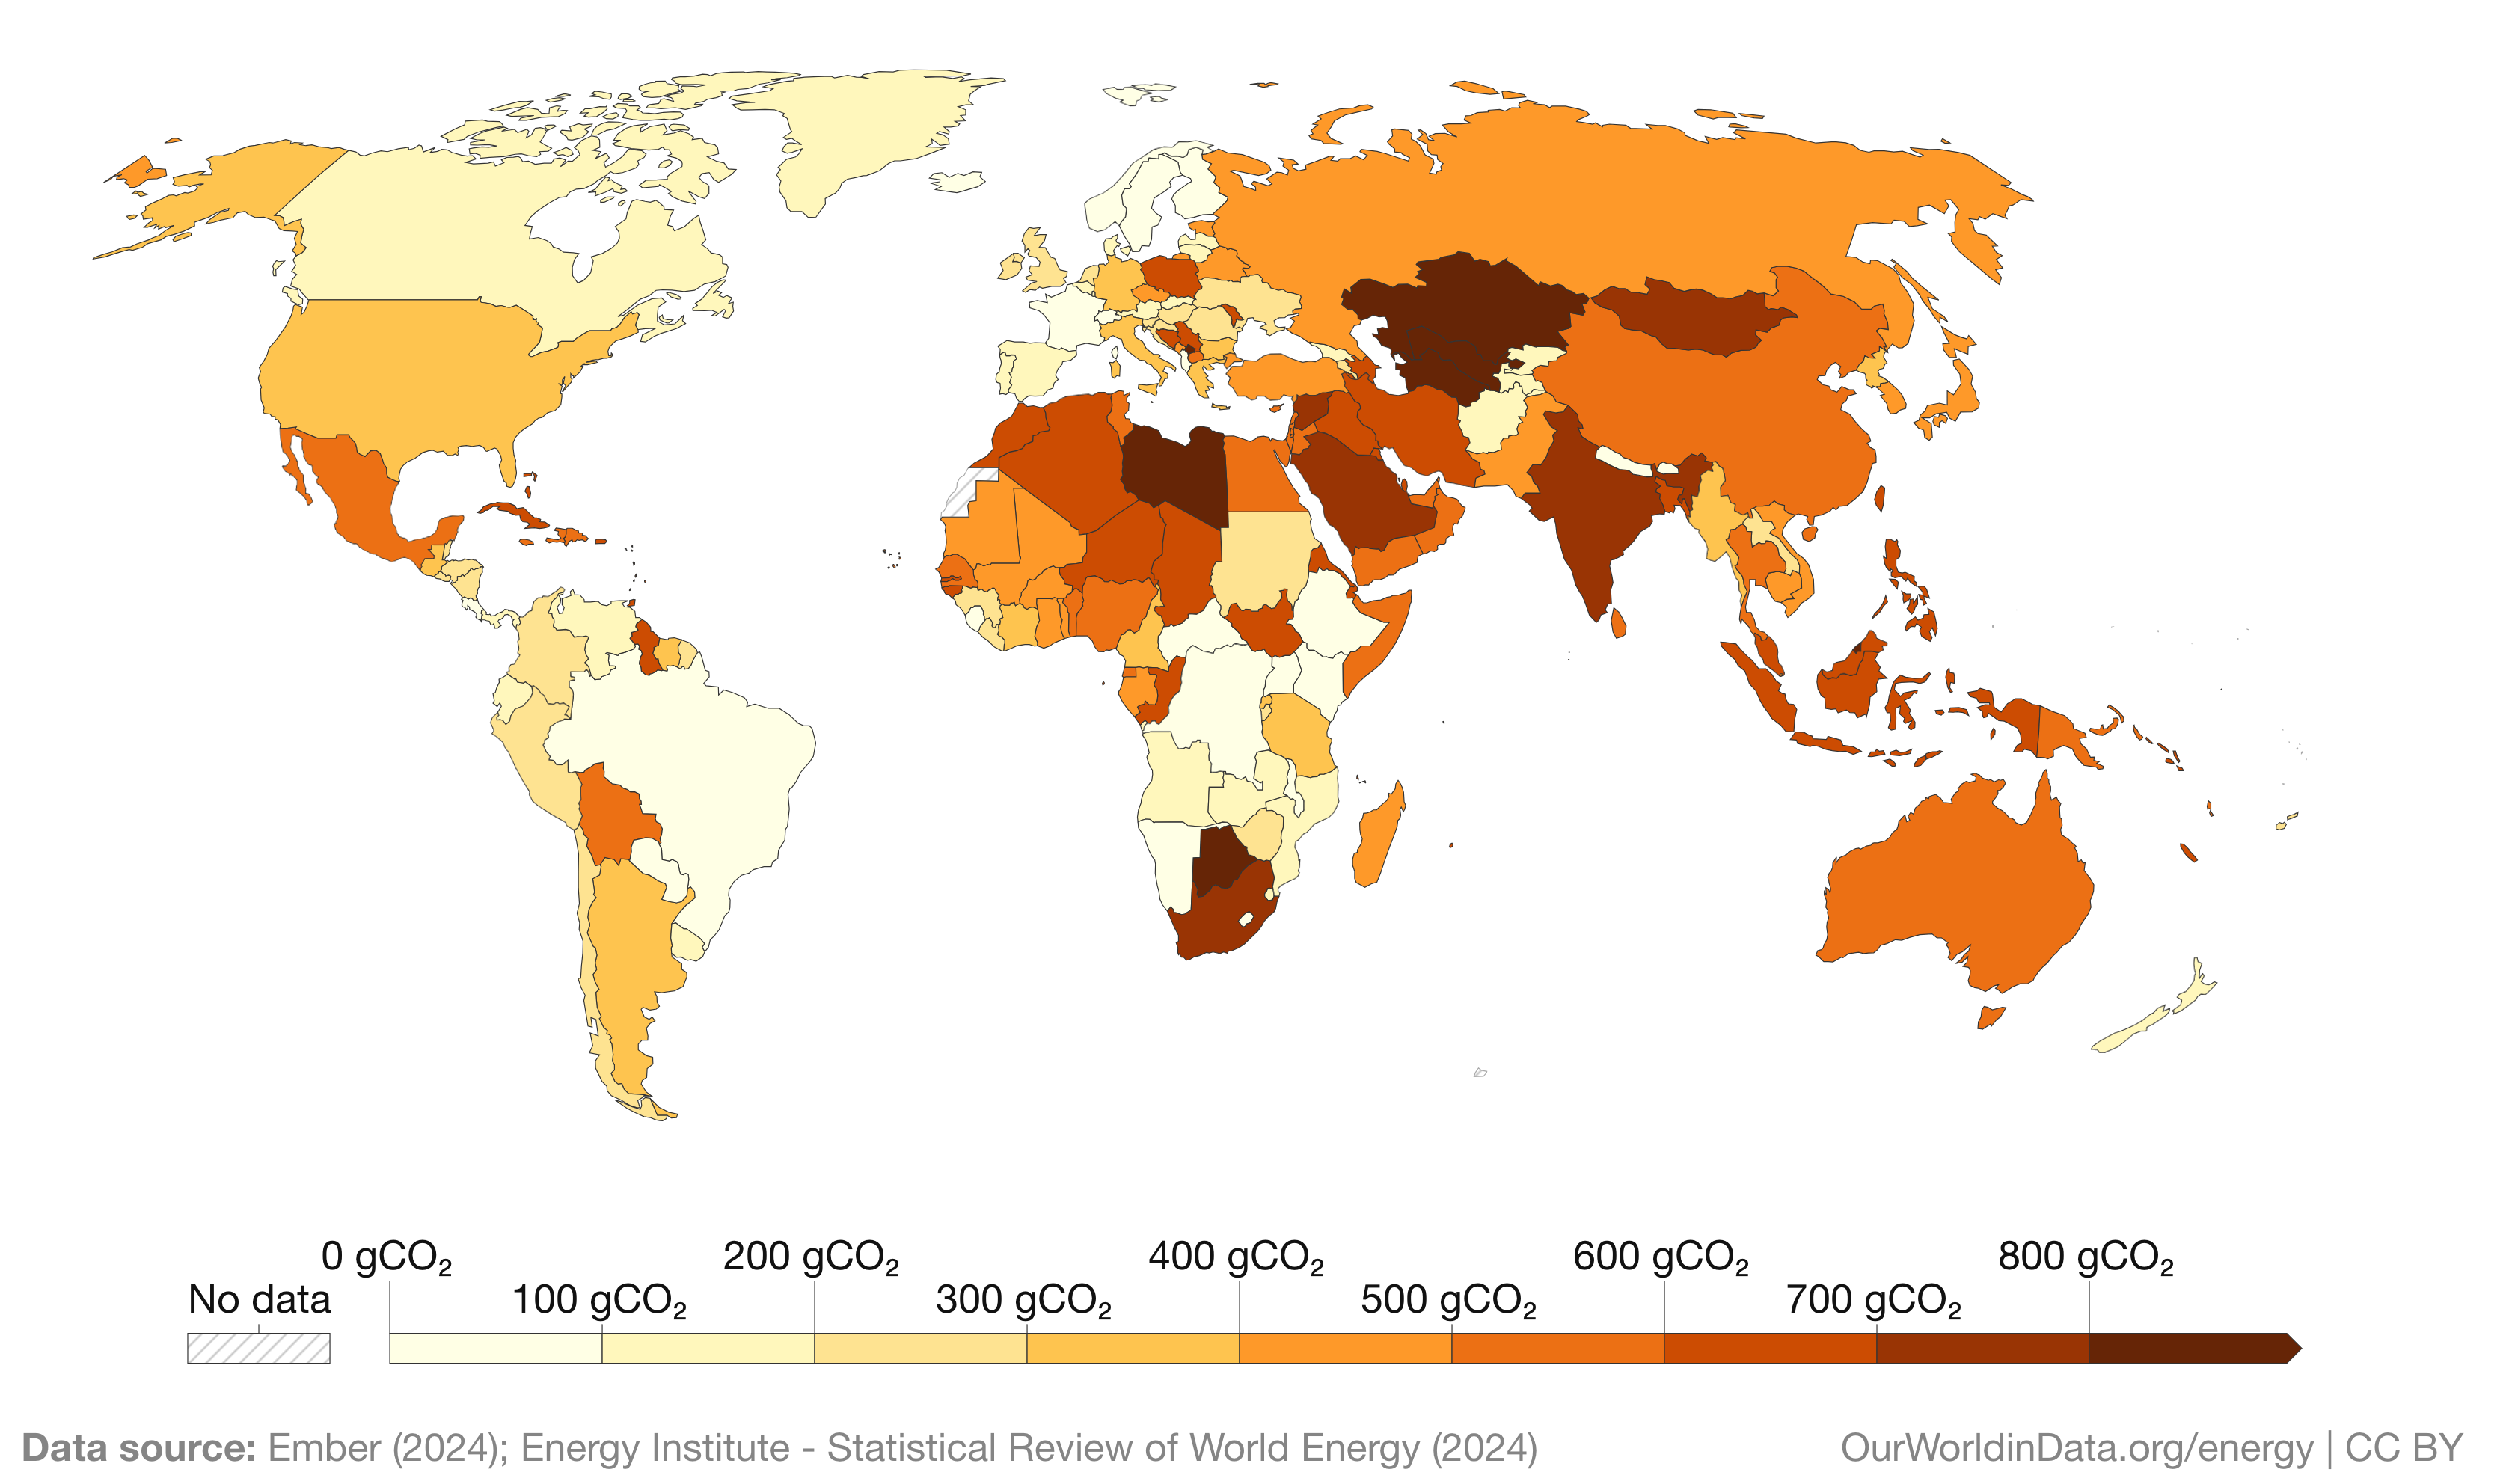
\includegraphics[width=\linewidth]{imgs/carbon-intensity-electricity.png}
    \caption{Carbon intensity of electricity generation, 2023. Source: \cite{ember2024carbonintensity}}
    \label{fig:carbon_intensity}
\end{figure}

By integrating real-time hardware usage monitoring with location-based carbon intensity data, CodeCarbon enables researchers 
and practitioners to quantify the environmental impact of their computations. This information can help guide decision-making, 
such as optimizing code efficiency, choosing lower-carbon data centers, or scheduling workloads during periods of higher renewable 
energy availability.

\section{Extending HADA with CodeCarbon}

\subsection{Energy Management Algorithms}

The first step in extending HADA to incorporate Carbon Intensity is to construct a dataset that includes carbon footprint data from 
algorithm execution. This requires integrating \textbf{CodeCarbon} into the computational workflow used for running algorithms. 

For this study, we analyzed two algorithms: \textbf{ANTICIPATE} and \textbf{CONTINGENCY}, originally introduced in 
\cite{ijcai2019p150, 10.1007/978-3-319-93031-2_8} and previously used in the HADA framework paper \cite{DEFILIPPO2022109199}. 
These algorithms belong to the domain of Energy Management Systems and are designed to compute the amount of energy 
that must be generated to meet a required load while minimizing the total energy cost over a daily time horizon. Both methods
consider the inherent uncertainty in energy demand and production.

\begin{itemize}
    \item \textbf{ANTICIPATE} is an \textit{online}, scenario-based anticipatory algorithm that adapts dynamically to uncertainty.
    \item \textbf{CONTINGENCY} is a hybrid \textit{offline/online} approach that first constructs (offline) a pool of solutions, 
    which is then used to guide an efficient online decision-making process.
\end{itemize}

Both methods are characterized by a tunable configuration parameter that can be adjusted based on performance constraints, 
particularly execution time and solution quality:
\begin{itemize}
    \item For \textbf{ANTICIPATE}, the configuration parameter is the number of considered \textit{scenarios} (\verb|nScenarios|).
    \item For \textbf{CONTINGENCY}, it is the number of \textit{traces} (\verb|nTraces|).
\end{itemize}

The goal of HADA is to learn the relationship between this configuration parameter and various performance metrics that characterize 
algorithm efficiency and resource usage. The original dataset used in HADA includes the following attributes:

\begin{itemize}
    \item \verb|nParam|: The configuration parameter of the algorithm (\verb|nScenarios| for ANTICIPATE, \verb|nTraces| for 
    CONTINGENCY).
    \item \verb|time(s)|: Execution time required to find a solution.
    \item \verb|sol(keuro)|: Cost of the obtained solution (expressed in thousand euros), serving as a measure of solution quality.
    \item \verb|memAvg(MB)|: Average memory usage of the algorithm (in MB).
\end{itemize}

\subsection{Incorporating Energy and Carbon Footprint Metrics}

To extend this approach, we integrated additional metrics related to \textbf{energy consumption} and \textbf{carbon footprint}, 
leveraging the capabilities of CodeCarbon. The following attributes were added to the dataset:

\begin{itemize}
    \item \verb|emissions|: Total $\mathsf{CO_2e}$ emissions generated during execution (kg).
    \item \verb|emission_rate|: Rate of $\mathsf{CO_2e}$ emissions per second (kg/s).
    \item \verb|cpu_energy|: Energy consumed by the CPU (kWh).
    \item \verb|ram_energy|: Energy consumed by RAM (kWh).
    \item \verb|tot_energy|: Total energy consumption (kWh), which is the sum of \verb|cpu_energy| and \verb|ram_energy|. If 
    applicable, it also includes GPU energy consumption.
    \item \verb|country| and \verb|region|: Geographic location where the computation took place, used to determine the carbon 
    intensity of electricity.
    \item \verb|cpu_count|: Number of CPU cores used.
\end{itemize}

Additionally, we implemented tracking for the peak memory usage of each execution, which we included in the dataset under the 
attribute:

\begin{itemize}
    \item \verb|memPeak(MB)|: Maximum memory usage (in MB) recorded during execution.
\end{itemize}

By incorporating these additional metrics, HADA can now model not only algorithm efficiency and solution quality but also the 
environmental impact of computational workloads. This enhancement allows for a more comprehensive optimization approach, balancing 
performance requirements with sustainability considerations.

\subsection{Min-Cut/Max-Flow Algorithms}

Following our initial experiments with ANTICIPATE and CONTINGENCY, which were already included in HADA, we sought to extend our 
study to a broader class of algorithms. We selected a set of algorithms used to solve the \textbf{Minimum Cut/Maximum Flow 
(Min-Cut/Max-Flow)} problem in graphs, a fundamental problem in combinatorial optimization with widespread applications in various 
domains, particularly in \textbf{Computer Vision}. 

The Min-Cut/Max-Flow problem involves computing the maximum amount of flow that can be sent from a designated source node to a 
ink node in a flow network, subject to capacity constraints on edges. The \textbf{Max-Flow} problem seeks to maximize the total 
flow, while the \textbf{Min-Cut} problem finds the smallest set of edges that, if removed, would disconnect the source from the sink. 
The Max-Flow problem and the Min-Cut problem are closely related, as stated by the \textbf{Max-Flow Min-Cut Theorem}, which asserts 
that the maximum flow value in a network is equal to the capacity of the minimum cut.

Min-Cut/Max-Flow algorithms are widely used in image segmentation, stereo vision, and other Computer Vision tasks where images are 
represented as graphs, and energy minimization techniques are applied to solve labeling problems. We referred to the work of Jensen 
et al. (2023) \cite{Jensen2023Maxflow}, which provides a comprehensive review of state-of-the-art Min-Cut/Max-Flow algorithms, 
evaluated on a large dataset of Computer Vision problems. 

\subsubsection{Selected Algorithms}

Based on the findings of Jensen et al., we focused on three well-known Min-Cut/Max-Flow algorithms, each representing different 
families of flow-based optimization methods:

\begin{itemize}
    \item \textbf{Boykov-Kolmogorov (BK)}
    \item \textbf{Excess Incremental Breadth First Search (EIBFS)}
    \item \textbf{Hochbaum's Pseudo-Flow (HPF)}
\end{itemize}

According to Jensen et al., Min-Cut/Max-Flow algorithms can be broadly classified into different families based on their approach 
to augmenting paths and flow computation. The \textbf{Boykov-Kolmogorov} (BK) algorithm \cite{bk2004maxflow} belongs to the \textbf{Augmenting Paths 
(AP)} family, which is one of the oldest methods for solving the Max-Flow problem. This family dates back to the classical 
\textbf{Ford-Fulkerson Algorithm} \cite{ford1956maxflow}, which introduced the concept of augmenting paths to iteratively 
increase the flow. BK extends this approach by introducing heuristic techniques to improve efficiency, making it particularly 
effective for Computer Vision applications.

On the other hand, \textbf{Excess Incremental Breadth First Search (EIBFS)} \cite{goldberg2015faster} and \textbf{Hochbaum’s 
Pseudo-Flow (HPF)} \cite{hochbaum2008pseudoflow} belong to the \textbf{Pseudoflow} family, which differs from augmenting path 
methods in the way it manages flow excess. These algorithms prioritize maintaining a valid preflow at all times and use alternative 
strategies to push flow across the network, often improving efficiency in large-scale instances. 

The main differences between these algorithm families lie in the order in which they traverse nodes while searching for augmenting 
paths and in their mechanisms for pushing flow along paths in the graph.

\subsubsection{Algorithm Variants Considered}

Unlike ANTICIPATE and CONTINGENCY, which have explicit tunable configuration parameters, these Min-Cut/Max-Flow algorithms can 
be implemented with different optimizations \cite{Jensen2023Maxflow}. We treated the specific implementation variant of each algorithm as a configuration 
parameter and considered the following versions:

\begin{itemize}
    \item \textbf{Boykov-Kolmogorov (BK) Variants:}
    \begin{itemize}
        \item \textbf{BK}: The reference implementation.
        \item \textbf{MBK}: An optimized version by Jensen et al., using indices instead of pointers to reduce memory footprint.
        \item \textbf{MBK-R}: A second optimized version that reorders arcs to ensure that all outgoing edges from a node are 
        stored contiguously in memory.
    \end{itemize}
    \item \textbf{Excess Incremental Breadth First Search (EIBFS) Variants:}
    \begin{itemize}
        \item \textbf{EIBFS}: A slightly modified version of the original EIBFS algorithm.
        \item \textbf{EIBFS-I}: A version that replaces pointers with indices to improve memory locality.
        \item \textbf{EIBFS-I-NR}: A version similar to EIBFS-I but without arc reordering.
    \end{itemize}
    \item \textbf{Hochbaum’s Pseudo-Flow (HPF) Variants:}
    \begin{itemize}
        \item \textbf{HPF-H-F}: Highest-label variant using FIFO buckets.
        \item \textbf{HPF-H-L}: Highest-label variant using LIFO buckets.
        \item \textbf{HPF-L-F}: Lowest-label variant using FIFO buckets.
        \item \textbf{HPF-L-L}: Lowest-label variant using LIFO buckets.
    \end{itemize}
\end{itemize}

\subsubsection{Energy and Carbon Footprint Monitoring}

Jensen et al. provided scripts to evaluate the runtime performance of these algorithms, measuring both initialization time and 
execution time. To extend this analysis with energy consumption and carbon footprint tracking, we modified their experimental 
setup by integrating \textbf{CodeCarbon}. 

Since the original implementations are written in C++, we wrapped the algorithm scripts with a Python interface to facilitate 
real-time monitoring. This wrapper was designed to:
\begin{itemize}
    \item Track memory usage throughout execution.
    \item Use CodeCarbon to measure CPU and RAM energy consumption.
    \item Record $\mathsf{CO_2e}$ emissions based on the energy consumption and Carbon Intensity of the execution environment.
\end{itemize}

Unlike the experiments with ANTICIPATE and CONTINGENCY, where solution quality was a critical performance metric, here we focus 
solely on computational efficiency. The primary metrics of interest for this study are execution time, memory consumption, energy 
consumption, and environmental impact. By incorporating these Min-Cut/Max-Flow algorithms into HADA, we aim to explore 
energy-efficient graph-based optimization techniques and further refine our approach to sustainable AI computation.

\chapter{Experimental Analysis}

\section{Benchmarking on Different Hardware Platforms}

To comprehensively evaluate the performance of the selected algorithms under varying computational environments, we conducted experiments on multiple hardware platforms. This approach allows 
us to better capture how changes in hardware configurations impact execution time, energy consumption, and carbon footprint.

\subsection{Experimental Setup}

The benchmark phase was carried out on the following computing environments:

\begin{itemize}
    \item \verb|mbp19|: A personal laptop running MacOS Ventura 13.6.7, equipped with:
    \begin{itemize}
        \item 1.4 GHz Quad-Core Intel Core i5 processor;
        \item 8 GB 2133 MHz LPDDR3 RAM.
    \end{itemize}
    
    \item \verb|PC|: A desktop computer running Ubuntu 24.4 LTS, featuring:
    \begin{itemize}
        \item 3.4 GHz Intel Core i7-4770 Quad-Core processor;
        \item 8 GB DDR3 RAM.
    \end{itemize}
    
    \item \verb|leonardo|: A high-performance computing (HPC) infrastructure, \textbf{Leonardo}, hosted by \textbf{CINECA}. Leonardo consists of 4992 computing nodes, distributed across 
    two primary partitions, i.e. the Booster Partition and the Data Centric General Purpose partition. For our benchmark, we will rely on the booster partition, which has the following 
    specifics:
    \begin{itemize}
        \item 512 GB (8 × 64 GB DDR4 3200 MHz) RAM per node;
        \item Single-socket, 32-core Intel Xeon Platinum 8358 CPU, 2.60 GHz (Ice Lake) (110,592 total cores);
        \item 4× NVIDIA custom Ampere A100 GPUs with 64 GB HBM2e memory, NVLink 3.0 (200 GB/s).
    \end{itemize}
\end{itemize}

Leonardo offers the possibility of launching jobs for execution on the booster partition using the slurm job scheduler, by specified the required runtime and resources. For the benchmark 
runs with anticipate and contingency, we requested 16 cores, while the min-cut/max-flow algorithm runs were executed on 32 cores.

\subsection{Benchmarking ANTICIPATE and CONTINGENCY}

For the first set of experiments, we executed \textbf{ANTICIPATE} and \textbf{CONTINGENCY} on a collection of 30 problem instances. These instances were sampled using a Gaussian statistical 
model, as proposed in \cite{DEFILIPPO2022109199}. 

Each algorithm was executed on every instance with a varying configuration parameter (i.e., the number of \textit{traces} for CONTINGENCY and \textit{scenarios} for ANTICIPATE), ranging 
from 1 to 100. These experiments were performed on both \verb|mbp19| and \verb|leonardo|. As a result, we generated a dataset containing:

\begin{equation}
    30 \times 100 \times 2 \times 2 = 12,000 \text{ entries}.
\end{equation}

This dataset captures execution time, memory consumption, energy usage, and carbon footprint across different algorithmic configurations and hardware platforms.

\subsection{Benchmarking Min-Cut/Max-Flow Algorithms}

To evaluate the performance of the selected \textbf{Min-Cut/Max-Flow} algorithms, we relied on the dataset provided by Jensen et al. (2023) \cite{Jensen2023Maxflow}. This dataset contains a 
diverse set of Min-Cut/Max-Flow problem instances from the field of Computer Vision, allowing for a thorough assessment of algorithmic efficiency in real-world applications. Jensen et al. also
provided reference implementations of the algorithms, which we used for benchmarking.

Since these implementations were written in \textbf{C++} (for BK and EIBFS) and \textbf{C} (for HPF), integrating energy consumption tracking posed a challenge. Currently, few tools are 
available for directly monitoring the energy footprint of compiled C/C++ code. % TODO: Expand this discussion in the Related Work section.

To address this issue, we developed a \textbf{Python wrapper script} that executes the C++/C implementations and integrates \textbf{CodeCarbon} for energy and emission tracking. The wrapper 
allows us to monitor:
\begin{itemize}
    \item Execution time and memory usage;
    \item CPU and RAM energy consumption;
    \item $\mathsf{CO_2e}$ emissions based on real-time energy monitoring and Carbon Intensity data.
\end{itemize}

\subsection{Execution Constraints and Limitations}

While our goal was to run the selected algorithms on all instances of the Jensen et al. dataset, several factors constrained the scope of our experiments:

\begin{itemize}
    \item \textbf{Compilation and Platform Limitations:} The BK and EIBFS implementations could not be compiled on \verb|mbp19| due to missing dependencies and a lack of support for MacOS. 
    To address this, we utilized an alternative system—\verb|PC|—running a lightweight Ubuntu distribution, enabling execution on additional hardware.
    
    \item \textbf{Memory Constraints:} Some problem instances in the dataset were too large to fit within the available system memory. Although it was technically possible to use a swap 
    partition to accommodate larger instances, this would have distorted memory usage measurements, as available monitoring tools record only RAM consumption and do not account for swapped memory.
    
    \item \textbf{Execution Time Considerations:} Given the extensive number of instances in the dataset, running all of them would have been prohibitively time-consuming. As a result, we 
    selected a representative subset of problem instances that allowed us to evaluate performance across a range of complexity levels without exceeding computational constraints.
\end{itemize}

By executing experiments across multiple hardware platforms and addressing challenges related to execution and monitoring, we constructed a dataset that provides insights into algorithmic 
efficiency, energy consumption, and carbon emissions. The following sections will analyze the results obtained from these experiments and explore the implications of integrating sustainability
metrics into algorithm selection and hardware dimensioning.

\subsection{ANTICIPATE and CONTINGENCY}

Following the completion of the benchmark phase, we analyze the resulting data to evaluate the carbon emissions and energy consumption of the ANTICIPATE and CONTINGENCY algorithms. This section 
presents a comparative analysis of their environmental impact across different hardware platforms.

\subsubsection{Carbon Emissions Analysis}

Figure~\ref{fig:ant_cont_emissions} displays the carbon emissions for ANTICIPATE and CONTINGENCY, categorized by hardware platform. The data reveals that emissions tend to be higher for the 
ANTICIPATE algorithm, particularly when executed on the \verb|leonardo| platform. Overall, the measured values remain relatively small, except for one notable outlier exceeding 0.020 kg of 
$\mathsf{CO_2e}$. Most emission values fall within the range $[0,0.005]$ kg.

\begin{figure}[h!]
    \centering
    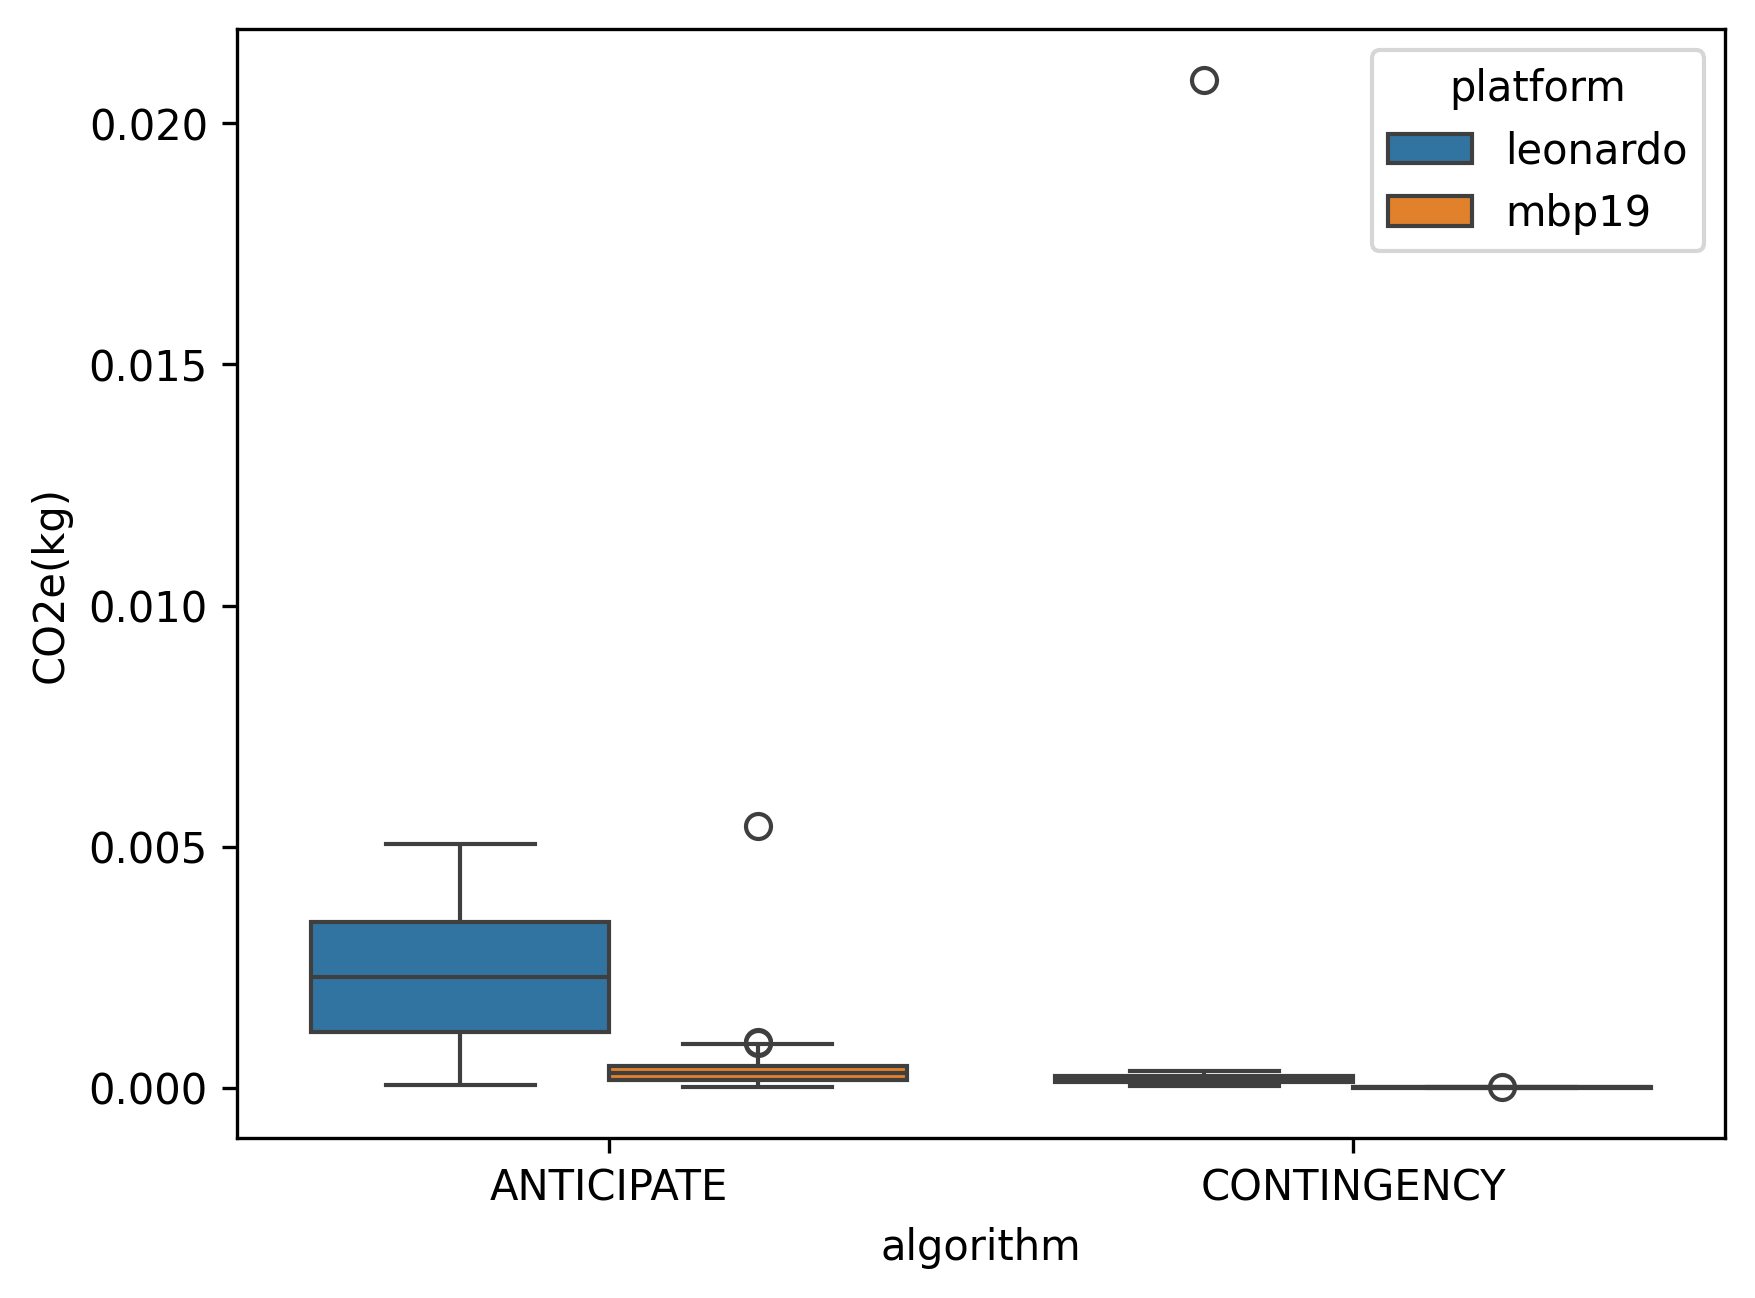
\includegraphics[width=0.8\textwidth]{imgs/emissions_ant_cont.png}
    \caption{CO$_2$ emissions for ANTICIPATE and CONTINGENCY across different platforms.}
    \label{fig:ant_cont_emissions}
\end{figure}

\subsubsection{Energy Consumption Analysis}

Similarly, Figure~\ref{fig:ant_cont_energy} illustrates the energy consumption for ANTICIPATE and CONTINGENCY. The overall trend aligns with the emissions data, with ANTICIPATE exhibiting higher 
energy consumption than CONTINGENCY, particularly on \verb|leonardo|, given that carbon emissions are directly proportional to energy usage in the absence of variation in Carbon Intensity.

\begin{figure}[h!]
    \centering
    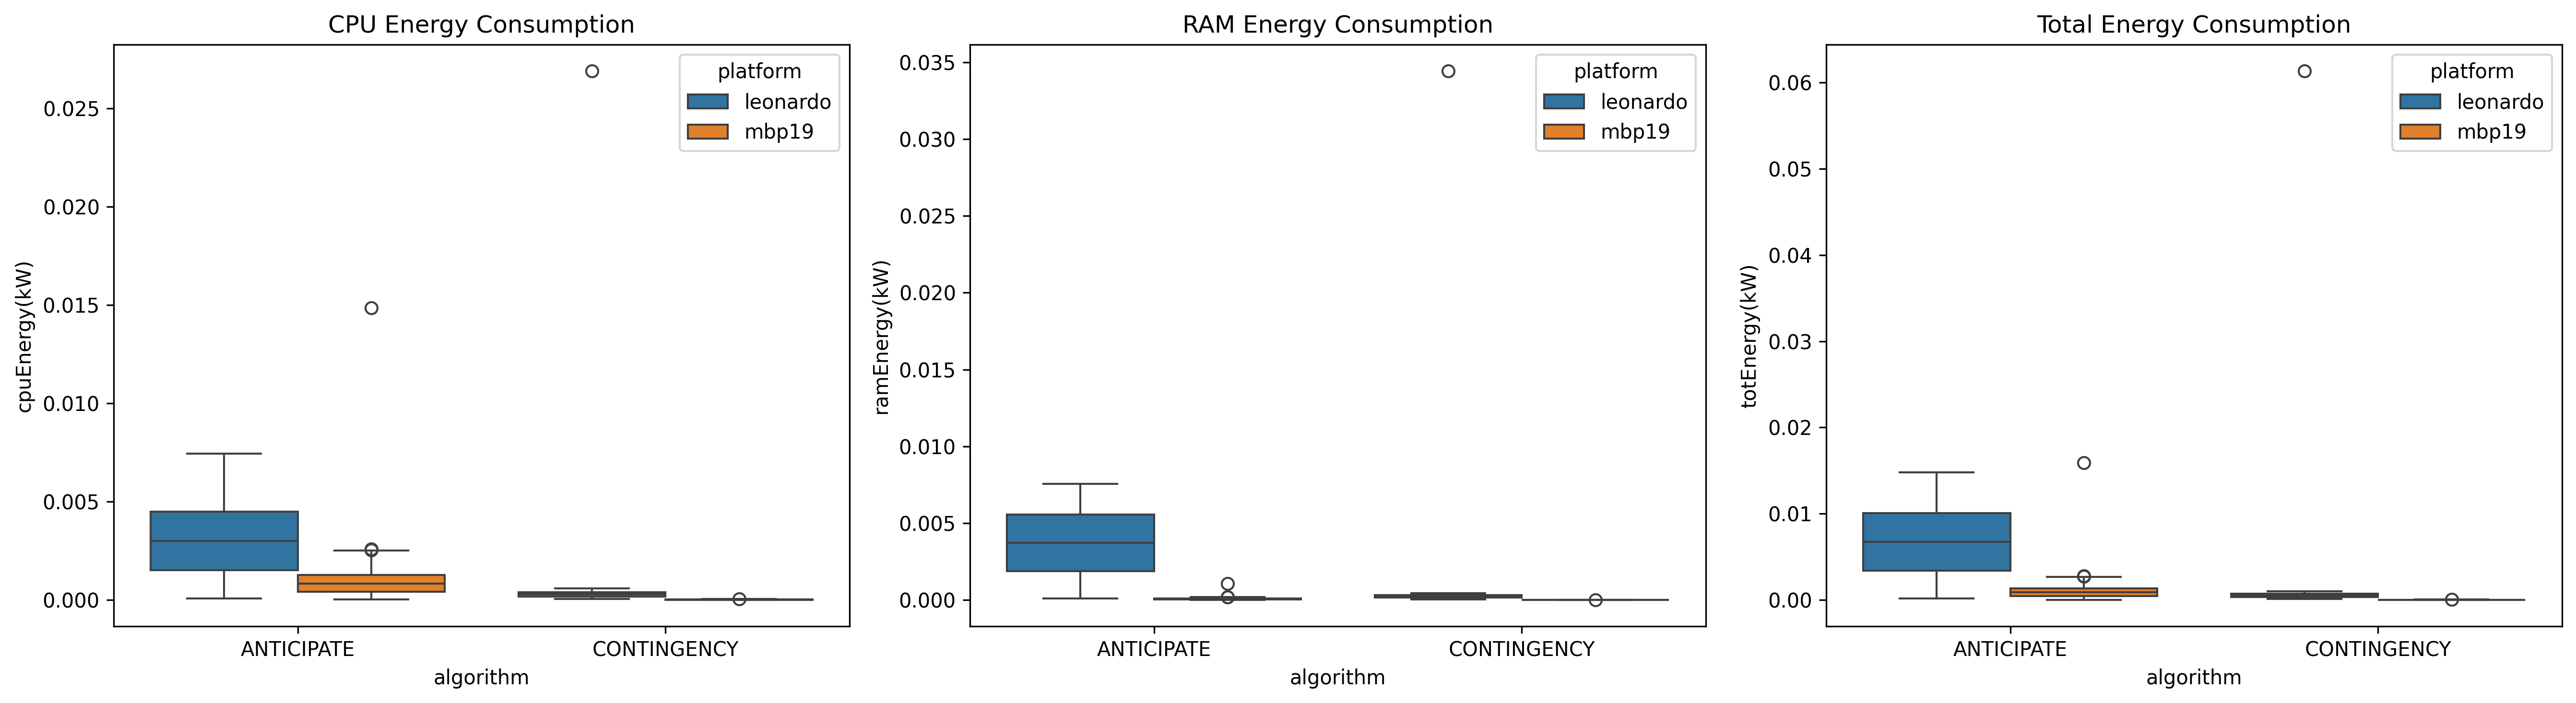
\includegraphics[width=\textwidth]{imgs/energy_ant_cont.png}
    \caption{Energy consumption for ANTICIPATE and CONTINGENCY across different platforms.}
    \label{fig:ant_cont_energy}
\end{figure}

\subsubsection{Correlation Analysis}

To further investigate the factors influencing emissions and energy consumption, Figure~\ref{fig:ant_corr_mat} and Figure~\ref{fig:cont_corr_mat} present the correlation matrices for ANTICIPATE and 
CONTINGENCY, respectively.

For ANTICIPATE (Figure~\ref{fig:ant_corr_mat}), the variable exhibiting the highest correlation with carbon emissions, aside from direct energy consumption, is the \textbf{average memory usage}, 
with a correlation coefficient of $0.93$. This suggests that higher memory consumption is a key contributor to increased emissions. Additionally, CPU energy consumption and RAM energy consumption 
both exhibit strong correlations with emissions, further reinforcing the relationship between computational resource usage and environmental impact.

\begin{figure}[h!]
    \centering
    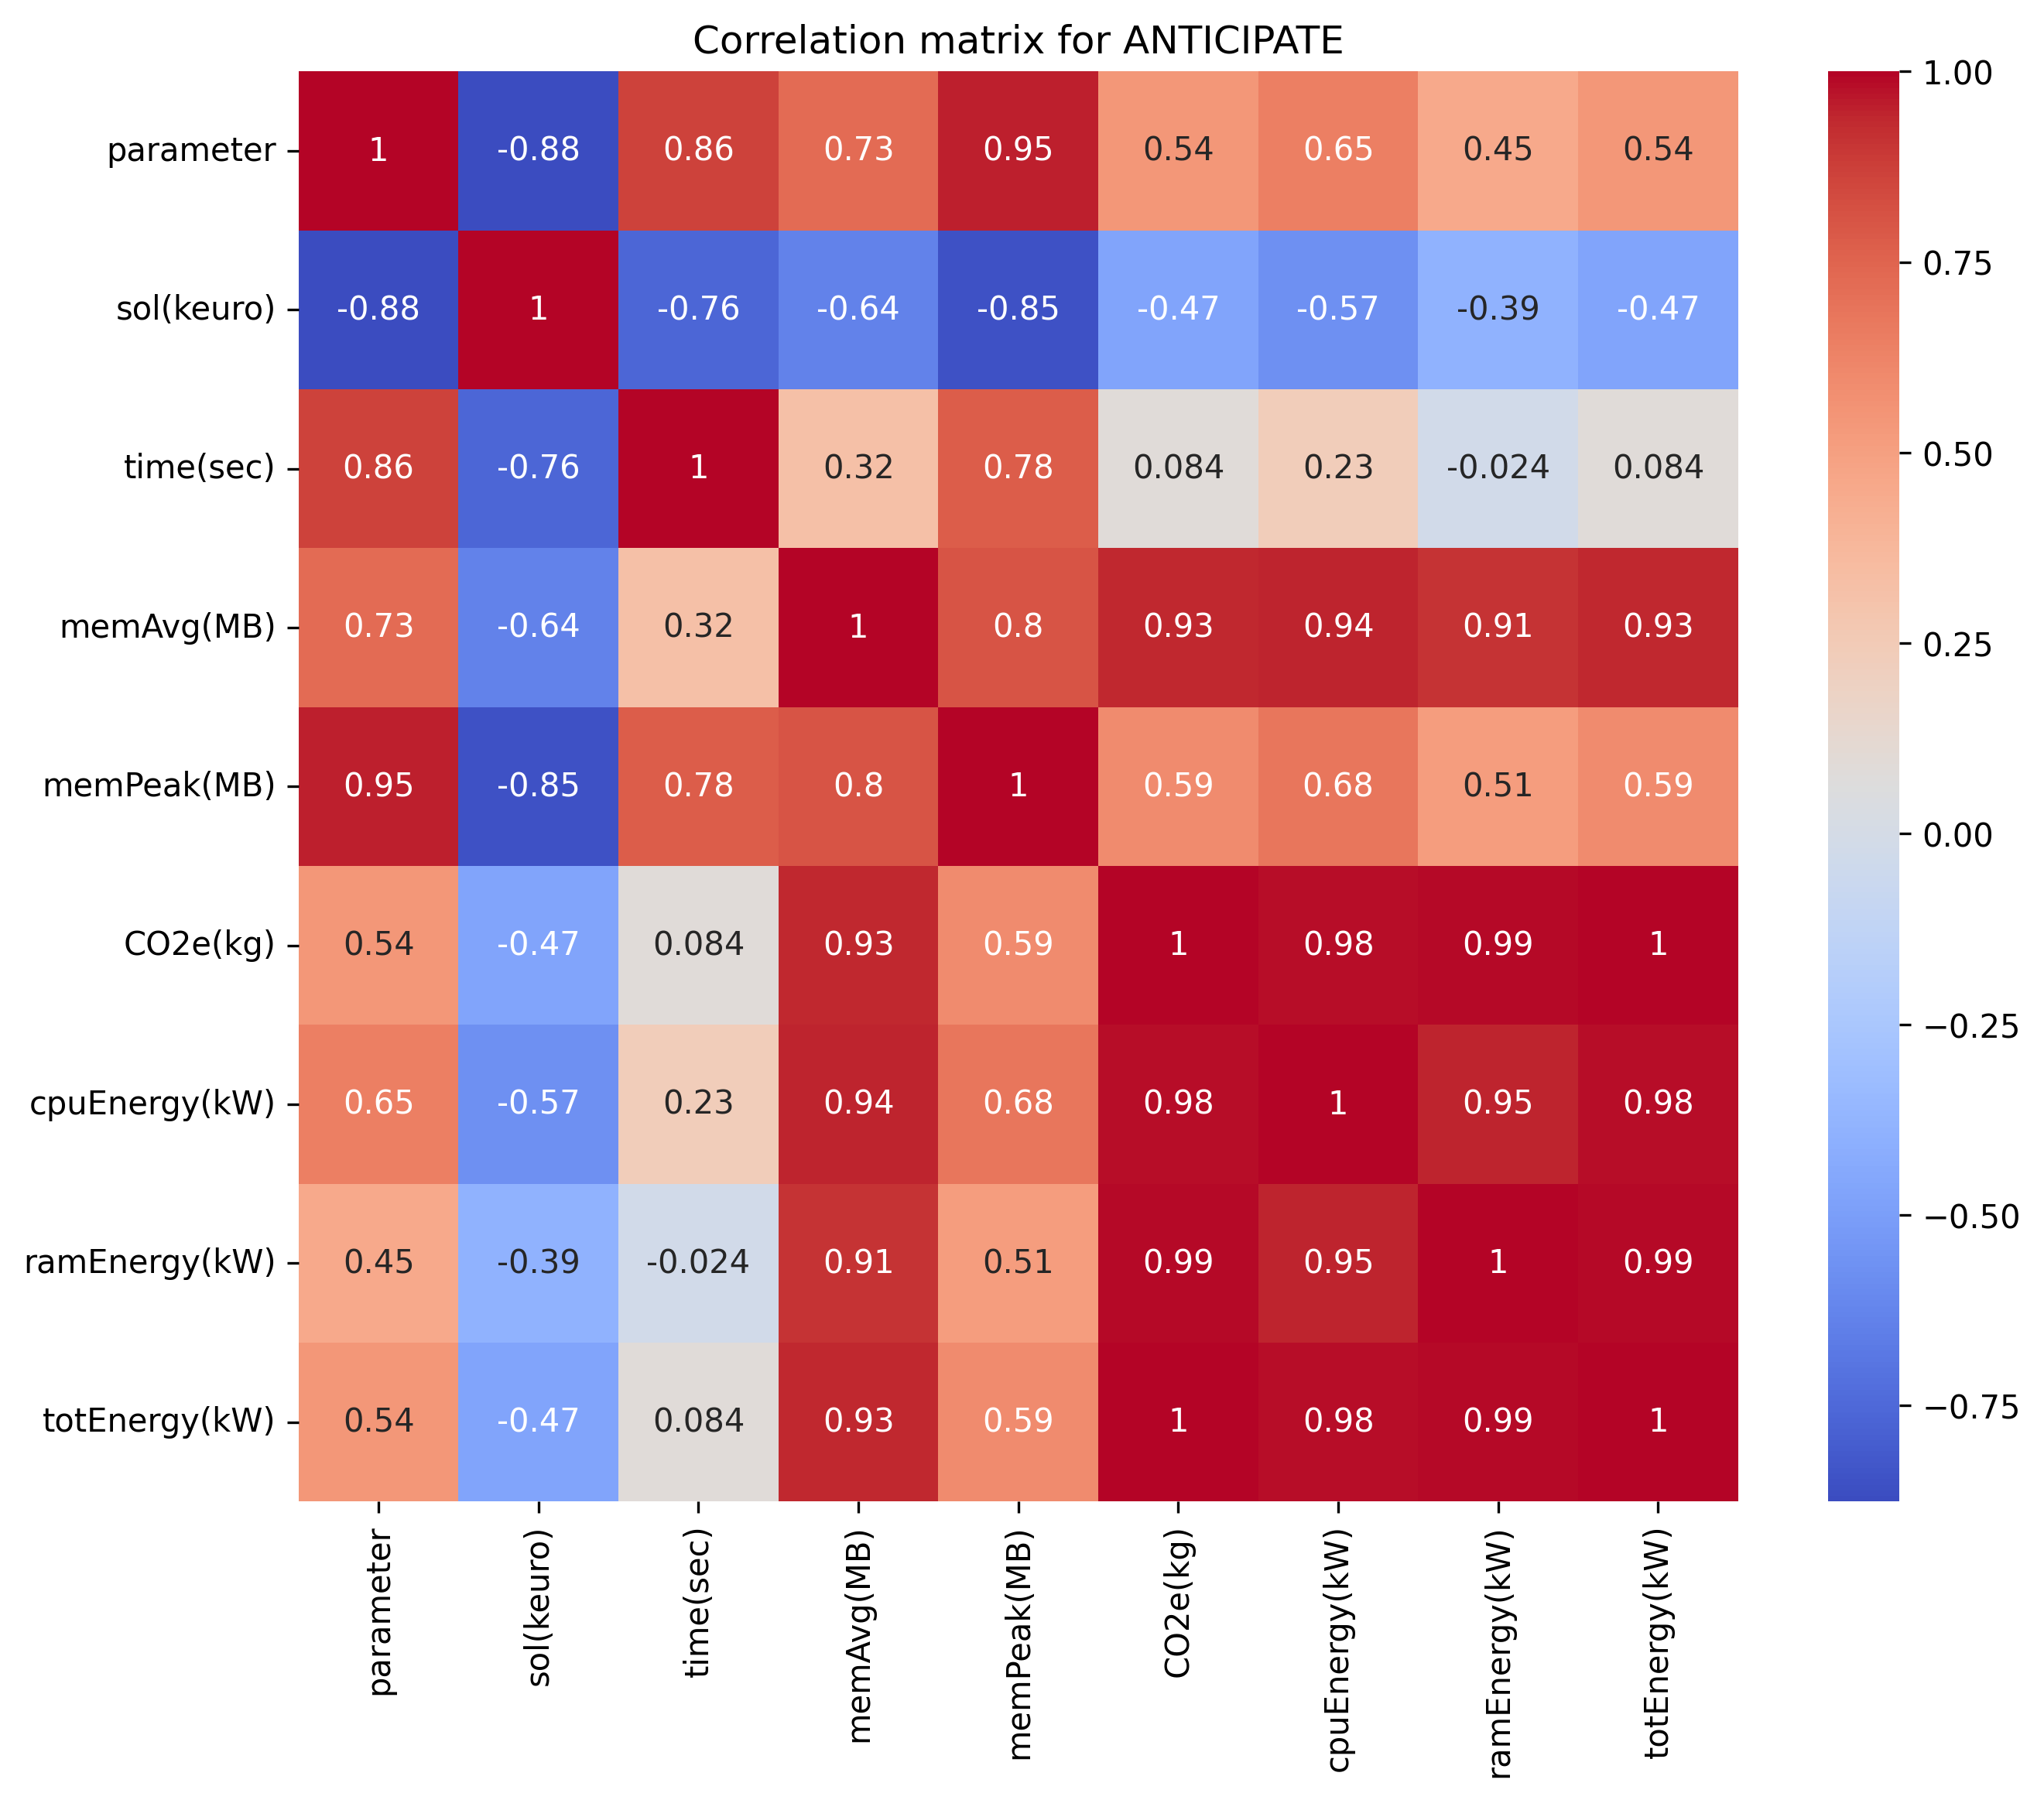
\includegraphics[width=0.8\textwidth]{imgs/ant_corr_mat.png}
    \caption{Correlation matrix for ANTICIPATE.}
    \label{fig:ant_corr_mat}
\end{figure}

In contrast, for CONTINGENCY (Figure~\ref{fig:cont_corr_mat}), there are no particularly strong linear correlations between emissions and other performance metrics. The highest correlation with 
emissions is observed for \textbf{execution time} ($0.36$), indicating that longer runtimes slightly contribute to higher emissions. However, the overall relationships appear weaker compared 
to ANTICIPATE, suggesting that CONTINGENCY’s energy usage is less dependent on a single dominant factor.

\begin{figure}[h!]
    \centering
    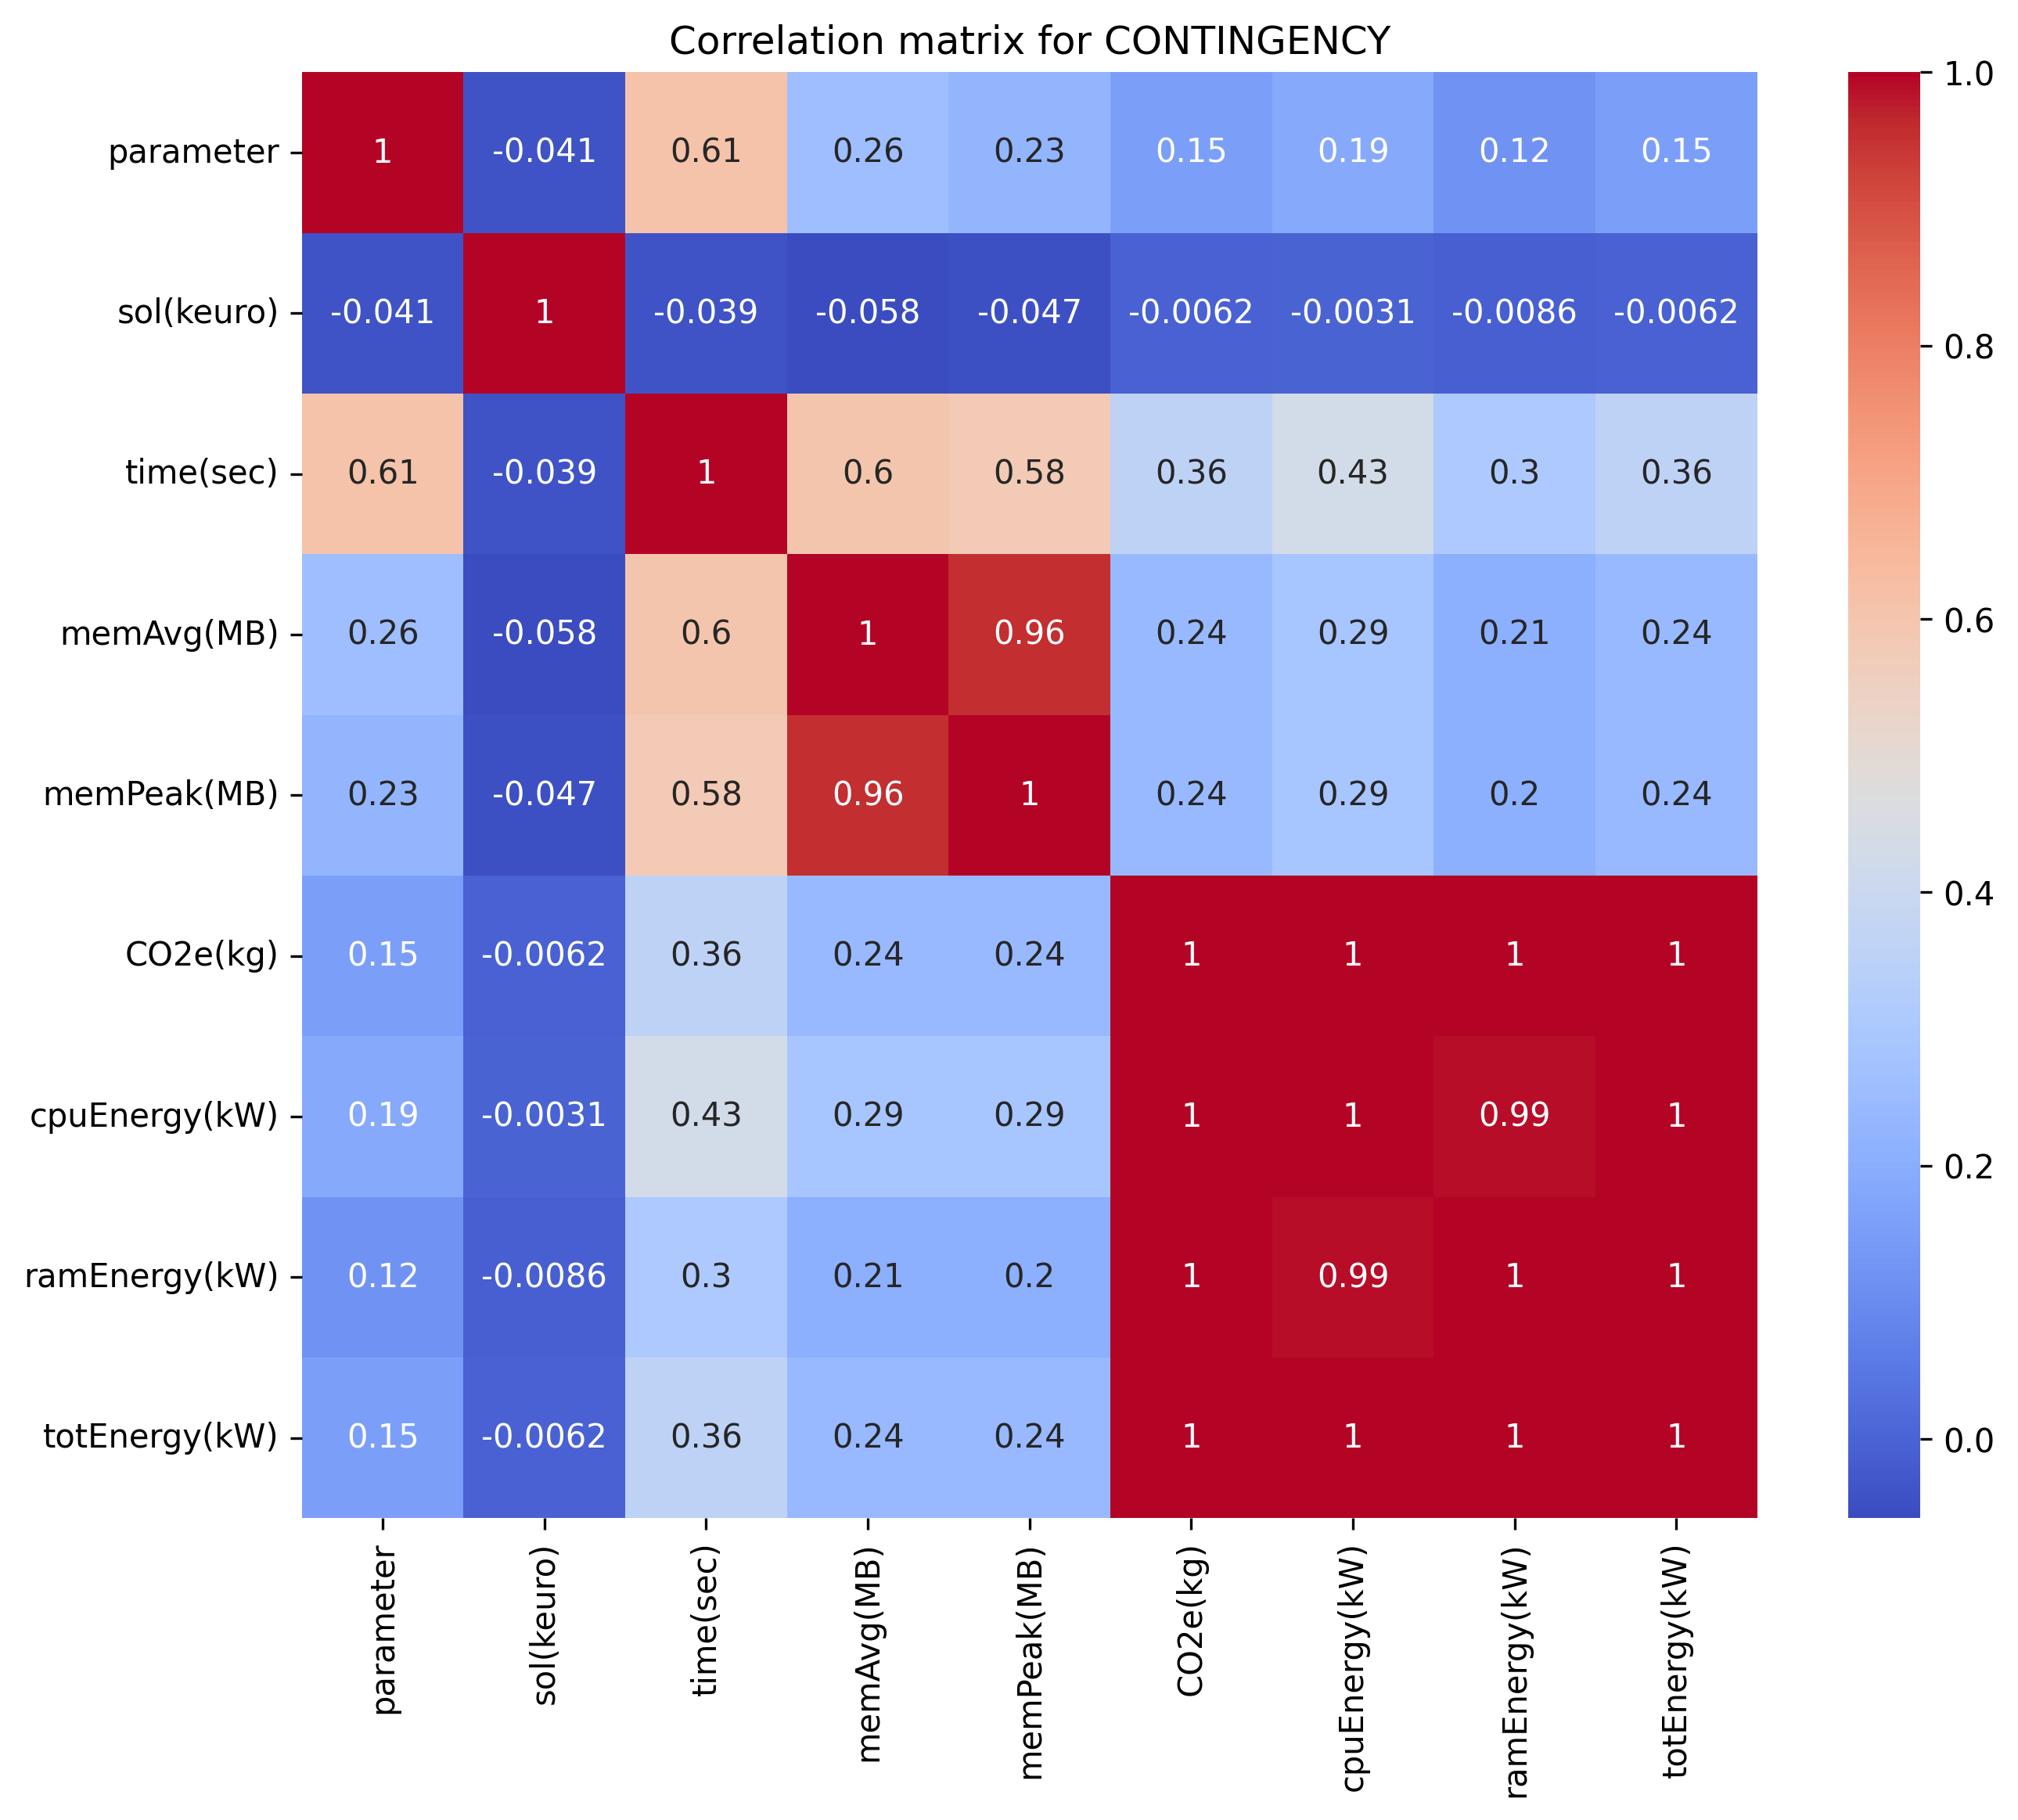
\includegraphics[width=0.8\textwidth]{imgs/cont_corr_mat.png}
    \caption{Correlation matrix for CONTINGENCY.}
    \label{fig:cont_corr_mat}
\end{figure}

From the correlation analysis, we make the following key observations:
\begin{itemize}
    \item Carbon emissions are perfectly proportional to total energy consumption, as indicated by the correlation of $1.0$ between \verb|totEnergy| and \verb|CO2e|. This reflects the fact 
    that, in the absence of varying Carbon Intensity, emissions are solely determined by energy consumption.
    \item Memory usage plays a significant role in determining emissions for ANTICIPATE, with a correlation of $0.93$. This suggests that optimizing memory allocation could be an effective s
    trategy for reducing emissions.
    \item For CONTINGENCY, execution time has the highest correlation with emissions ($0.36$), indicating a weaker but notable relationship.
    \item CPU and RAM energy consumption are highly correlated with total emissions ($0.98$ and $0.99$, respectively). Since total energy consumption is simply the sum of CPU and RAM energy, 
    this is expected.
    \item Retaining energy consumption values in the dataset is beneficial as these values can be scaled based on different Carbon Intensity factors. This enables an analysis of the impact 
    of computing in different geographic locations.
\end{itemize}

\subsubsection{Testing the HADA Framework with the Expanded Datasets}

To further explore the optimization capabilities of HADA, we conducted additional experiments on ANTICIPATE and CONTINGENCY, incorporating constraints on runtime, memory usage, and 
solution cost. The goal was to determine whether HADA could effectively optimize carbon emissions while satisfying various computational constraints. 

The results for ANTICIPATE are presented in Table \ref{tab:anticipate_results}. We tested multiple combinations of constraints on solution cost (expressed in thousands of euros, k€) and 
average memory consumption (expressed in MB), while minimizing CO$_2$ emissions (expressed in kg). In cases where HADA was unable to find a valid solution satisfying the constraints, we 
marked the corresponding results as "none".

\begin{table}[h!]
    \centering
    \begin{tabular}{|cc|ccccc|}
        \hline
        \multicolumn{2}{|c|}{Bounds} & \multicolumn{5}{c|}{Solution} \\
        \hline
        Mem (MB) & Cost (k€) & $n^P$ & HW & CO$_2$ (kg) & Mem (MB) & Cost (k€) \\
        \hline
        no & no & 1 & mbp19 & $7.23 \times 10^{-6}$ & - & - \\
        80 & no & none & none & none & none & none \\
        no & $100$ & none & none & none & none & none \\
        100 & $300$ & none & none & none & none & none \\
        150 & $300$ & 64 & mbp19 & $3.75 \times 10^{-4}$ & $141.53$ & $299.46$ \\
        170 & $270$ & 97 & mbp19 & $5.70 \times 10^{-4}$ & $169.85$ & $267.39$ \\
        170 & $280$ & 87 & mbp19 & $5.10 \times 10^{-4}$ & $160.12$ & $276.86$ \\
        300 & $500$ & 1 & mbp19 & $7.23 \times 10^{-6}$ & $81.47$ & $368.73$ \\
        \hline
    \end{tabular}
    \caption{Experimental results for the ANTICIPATE algorithm with constraints on the Average Memory usage and Solution Cost.}
    \label{tab:anticipate_results}
\end{table}

The results indicate that in most cases, minimizing CO$_2$ emissions aligns with minimizing memory consumption. The smallest emissions were observed when HADA selected configurations with fewer
scenarios ($n^P$). This is consistent with our earlier observations, where ANTICIPATE's carbon footprint was highly correlated with memory usage ($0.93$ correlation). We can also observe how
for tighter solution cost bounds, the numbber of scenarios tends to increase (reflecting the negative correlation of $-0.88$ as we can see in Figure~\ref{fig:ant_corr_mat}), and since increasing the 
number of scenarios means more memory usage, the carbon emissions also grows. When the solution cost is allowed to be higher, the number of scenarios is instead kept as low as possible, given
that we are trying to minimize the CO$_2$ emissions. Thus, in the case of ANTICIPATE we have a trade-off between CO$_2$ emissions and Solution cost.

A notable outcome is that, when trying to minimize the emissions HADA always selected the mbp19 platform. This suggests that the additional computational power offered by leonardo comes with an
higher energy cost, as shown by Figure~\ref{fig:ant_cont_emissions} and Figure~\ref{fig:ant_cont_energy}, so that, when the focus is on minimizing the CO$_2$ emissions mbp19 seems to be the "greener" choice.
The advanges of using leonardo may come instead from the reduced runtimes.

\begin{figure}[h!]
    \centering
    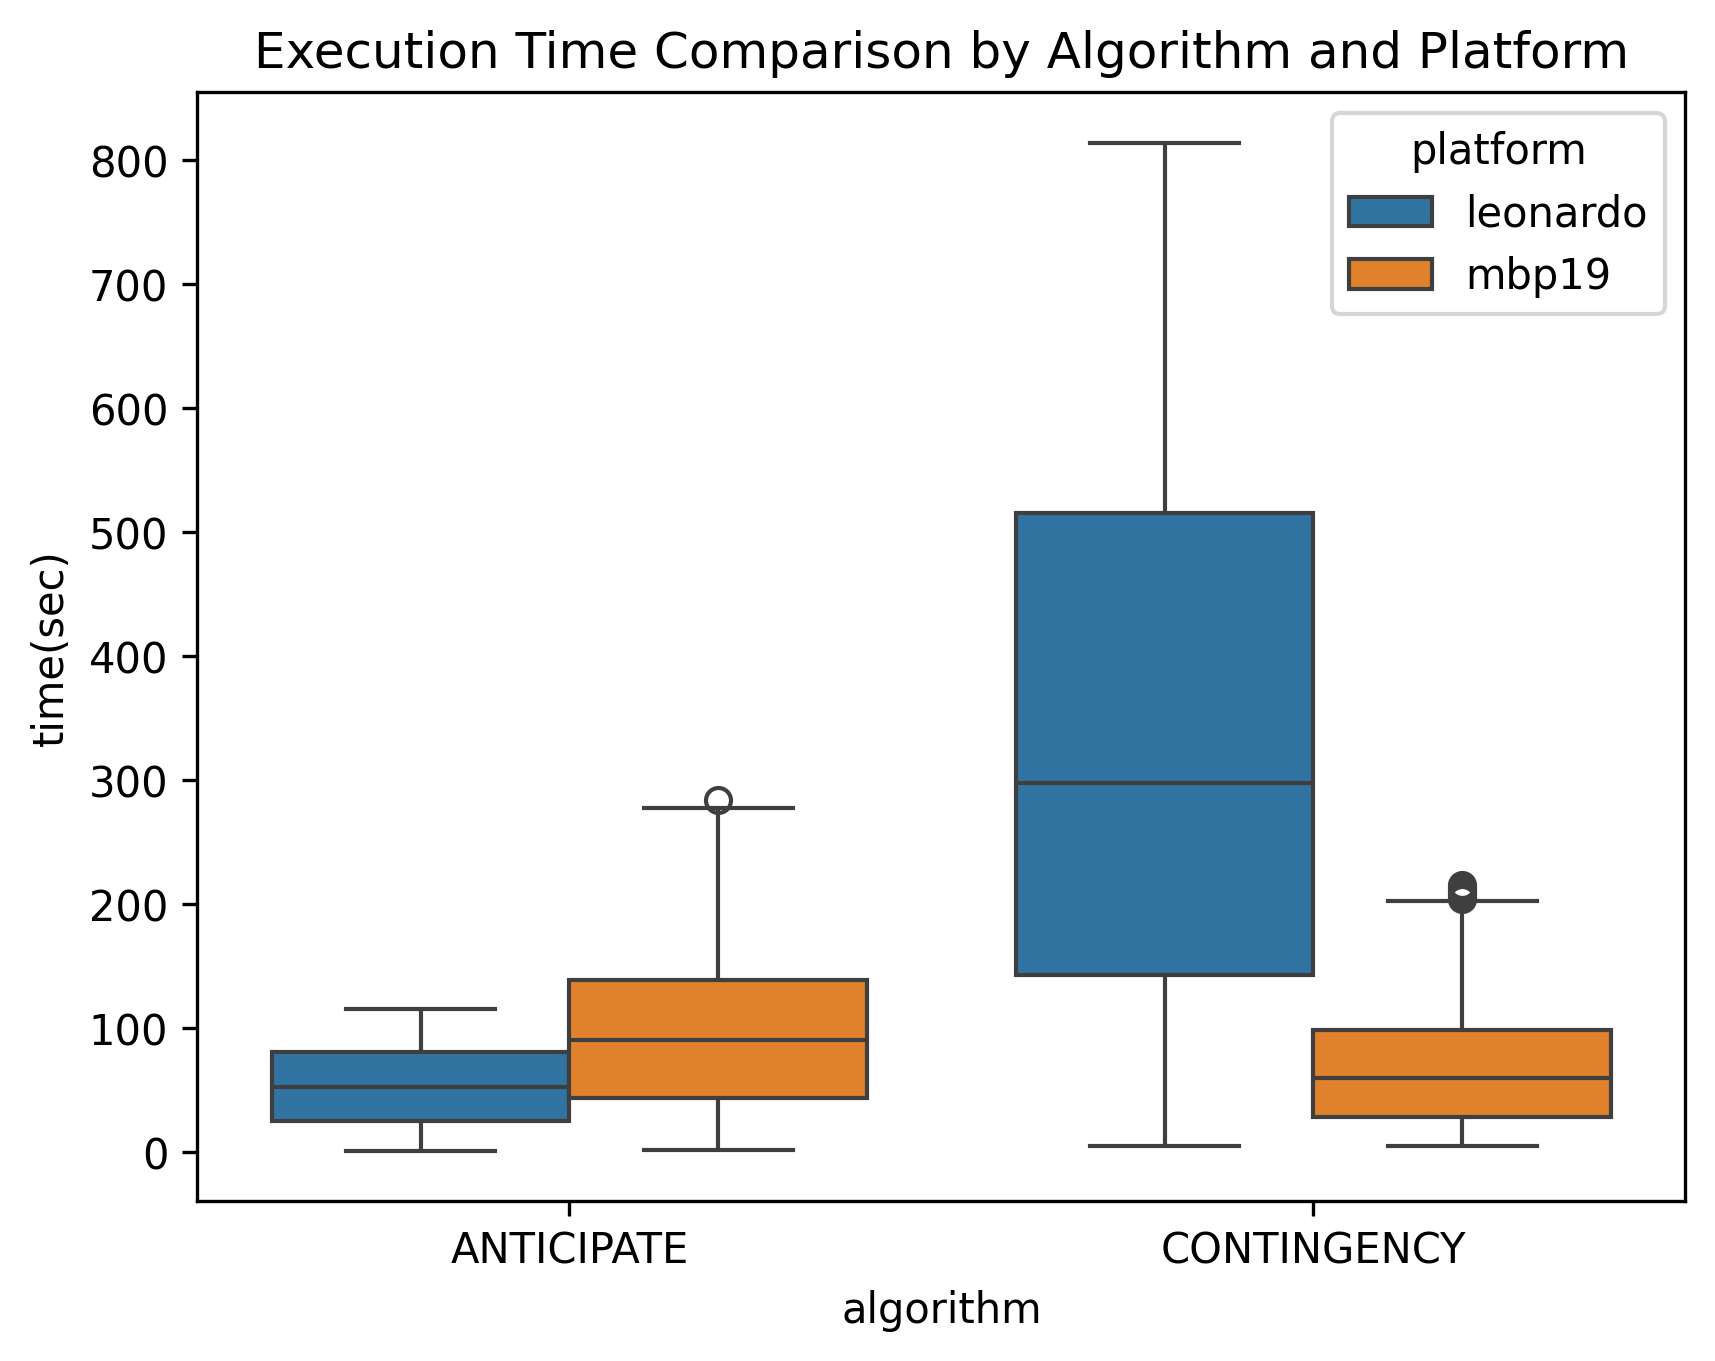
\includegraphics[width=0.8\textwidth]{imgs/time_comparison.png}
    \caption{Time Comparison between ANTICIPATE and CONTINGENCY on leonardo and mbp19}
    \label{fig:time_comparison}
\end{figure}

\ref{fig:time_comparison} shows that, for ANTICIPATE, the execution time time on leonardo is smaller on average, which is confirmed by \ref{tab:anticipate_runtime_comparison}

\begin{table}[h]
    \centering
    \begin{tabular}{llccccccc}
        \toprule
        \textbf{Algorithm} & \textbf{Platform} & \textbf{Mean} & \textbf{Std} & \textbf{Min} & \textbf{Max} \\
        \midrule
        \textbf{ANTICIPATE} & leonardo & 52.876531 & 31.205927 & 1.22 & 115.18 \\
                            & mbp19    & 93.023027 & 57.730152 & 1.50 & 284.29 \\
        \bottomrule
    \end{tabular}
    \caption{Comparison of runtime statistics for the ANTICIPATE algorithm on different platforms.}
    \label{tab:anticipate_runtime_comparison}
\end{table}

We can try to test the potential benefits of leonardo by using the runtime as objective to minimize in HADA. \ref{tab:anticipate_results_runtime} presents the results of a set of experiments 
with the objective of runtime minimization of ANTICIPATE, with constrinats on the solution cost and the CO$_2$ emissions.

\begin{table}[h!] 
    \centering
    \begin{tabular}{|cc|ccccc|}
        \hline
        \multicolumn{2}{|c|}{Bounds} & \multicolumn{5}{c|}{Solution} \\
        \hline
        CO2eq (kg) & Cost (k€) & $n^P$ & HW & CO$_2$ (kg) & Time (s) & Cost (k€) \\
        \hline
        0.005 & 300 & 60 & leonardo & $2.94 \times 10^{-3}$ & $62.63$ & $299.92$ \\
        0.01 & 280 & 87 & leonardo & $4.24 \times 10^{-3}$ & $92.04$ & $274.01$ \\
        0.1 & 270 & 96 & leonardo & $4.74 \times 10^{-3}$ & $100.94$ & $267.40$ \\
        0.0001 & 400 & 1 & leonardo & $7.53 \times 10^{-5}$ & $1.24$ & $368.73$ \\
        0.00001 & 400 & 1 & mbp19 & $7.23 \times 10^{-6}$ & $1.53$ & $368.73$ \\
        \hline
    \end{tabular}
    \caption{Experimental results for the ANTICIPATE algorithm, minimizing runtime with constraints on solution cost and CO2 emissions}
    \label{tab:anticipate_results_runtime}
\end{table}

From these experiments we can see that when we try to minimize the runtime, and we have tight bounds on the solution cost, the preferrable choice is leonardo, with an high number of scenarios. 
So this confirms that leonardo can actually provide advantages when the emphasis is on runtime minimization and constraints on the solution cost, since to obtain cheaper solutions a higher number
of scenarios is required, and this cause an increase in the runtime. For example, we can compare the runtimes of ANTICIPATE with 96 scenarios on both platforms, and we can see that on mbp19 they
are considerably higher (See \ref{tab:96_scenarios_runtime}):

\begin{table}[h]
    \centering
    \begin{tabular}{cccccccc}
        \hline
        \textbf{Platform} & \textbf{Mean} & \textbf{Std} & \textbf{Min} & \textbf{Max} \\
        \hline
        leonardo & 101.663448 & 2.280052 & 96.47 & 106.40 \\
        mbp19    & 184.732667 & 23.545764 & 167.55 & 256.84 \\
        \hline
    \end{tabular}
    \caption{Runtime statistics for 96 scenarios using the ANTICIPATE algorithm.}
    \label{tab:96_scenarios_runtime}
\end{table}

However, for the same configuration of the algorithm on mbp19, the emission values are an order of magnitude lower. Indeed, when constraints on the carbon emissions are very 
low ($ 1 \times 10 ^ {-5}$ or less), HADA starts preferring mbp19 to leonardo, due to the greater energy efficiency for smaller values of the parameter,
at the expense of an higher solution cost.

For CONTINGENCY, Table \ref{tab:contingency_results} presents the results of optimizing CO$_2$ emissions under constraints on execution time and solution cost. Given that execution time 
showed the highest correlation with emissions ($0.47$), we focused on determining whether limiting runtime would impact emissions optimization.

\begin{table}[h!]
    \centering
    \begin{tabular}{|cc|ccccc|}
        \hline
        \multicolumn{2}{|c|}{Bounds} & \multicolumn{5}{c|}{Solution} \\
        \hline
        Time (s) & Cost (k€) & $n^P$ & HW & CO$_2$ (kg) & Time (s) & Cost (k€) \\
        \hline
        no & no & 2 & mbp19 & $1.29 \times 10^{-6}$ & - & - \\
        no & $350$ & 4 & mbp19 & $1.53 \times 10^{-6}$ & - & $338.23k$ \\
        10 & no & 2 & mbp19 & $1.29 \times 10^{-6}$ & $6.01$ & - \\
        10 & $320$ & none & none & none & none & none \\
        60 & $350$ & 4 & mbp19 & $1.29 \times 10^{-6}$ & $7.68$ & $338.23$ \\
        120 & $320$ & 90 & mbp19 & $1.24 \times 10^{-5}$ & $119.47$ & $314.11$ \\
        \hline
    \end{tabular}
    \caption{Experimental results for the CONTINGENCY algorithm with constraints on runtime and solution cost.}
    \label{tab:contingency_results}
\end{table}

The results for CONTINGENCY further reinforce the platform selection pattern seen in ANTICIPATE: HADA consistently favored mbp19 over Leonardo. This was expected, as we can see In
\ref{fig:time_comparison}, that CONTINGENCY runs significantly slower on Leonardo than on mbp19. By looking at the dataset, we can see that Leonardo incurred a large overhead ($\approx60$s) 
even for a single trace, whereas mbp19 handled one trace in $5$-$6$s. This trend continued as traces increased, as with 100 traces, mbp19 has runtimes around 140 seconds, while leonardo runtime
values are around 800 seconds. Thus, contrary to what happened with ANTICIPATE, with CONTINGENCY using leonardo did not brought any significant advantage in performance. Even by looking at the
memory consumption we can see that mbp19 outperforms leonardo(\ref{fig:mem_usage_comparison}), with actually no visible gains in terms of solution cost, as we can see by Figure~\ref{fig:cost_comparison}. 

\begin{figure}[h!]
    \centering
    \begin{subfigure}[b]{0.4\linewidth}
        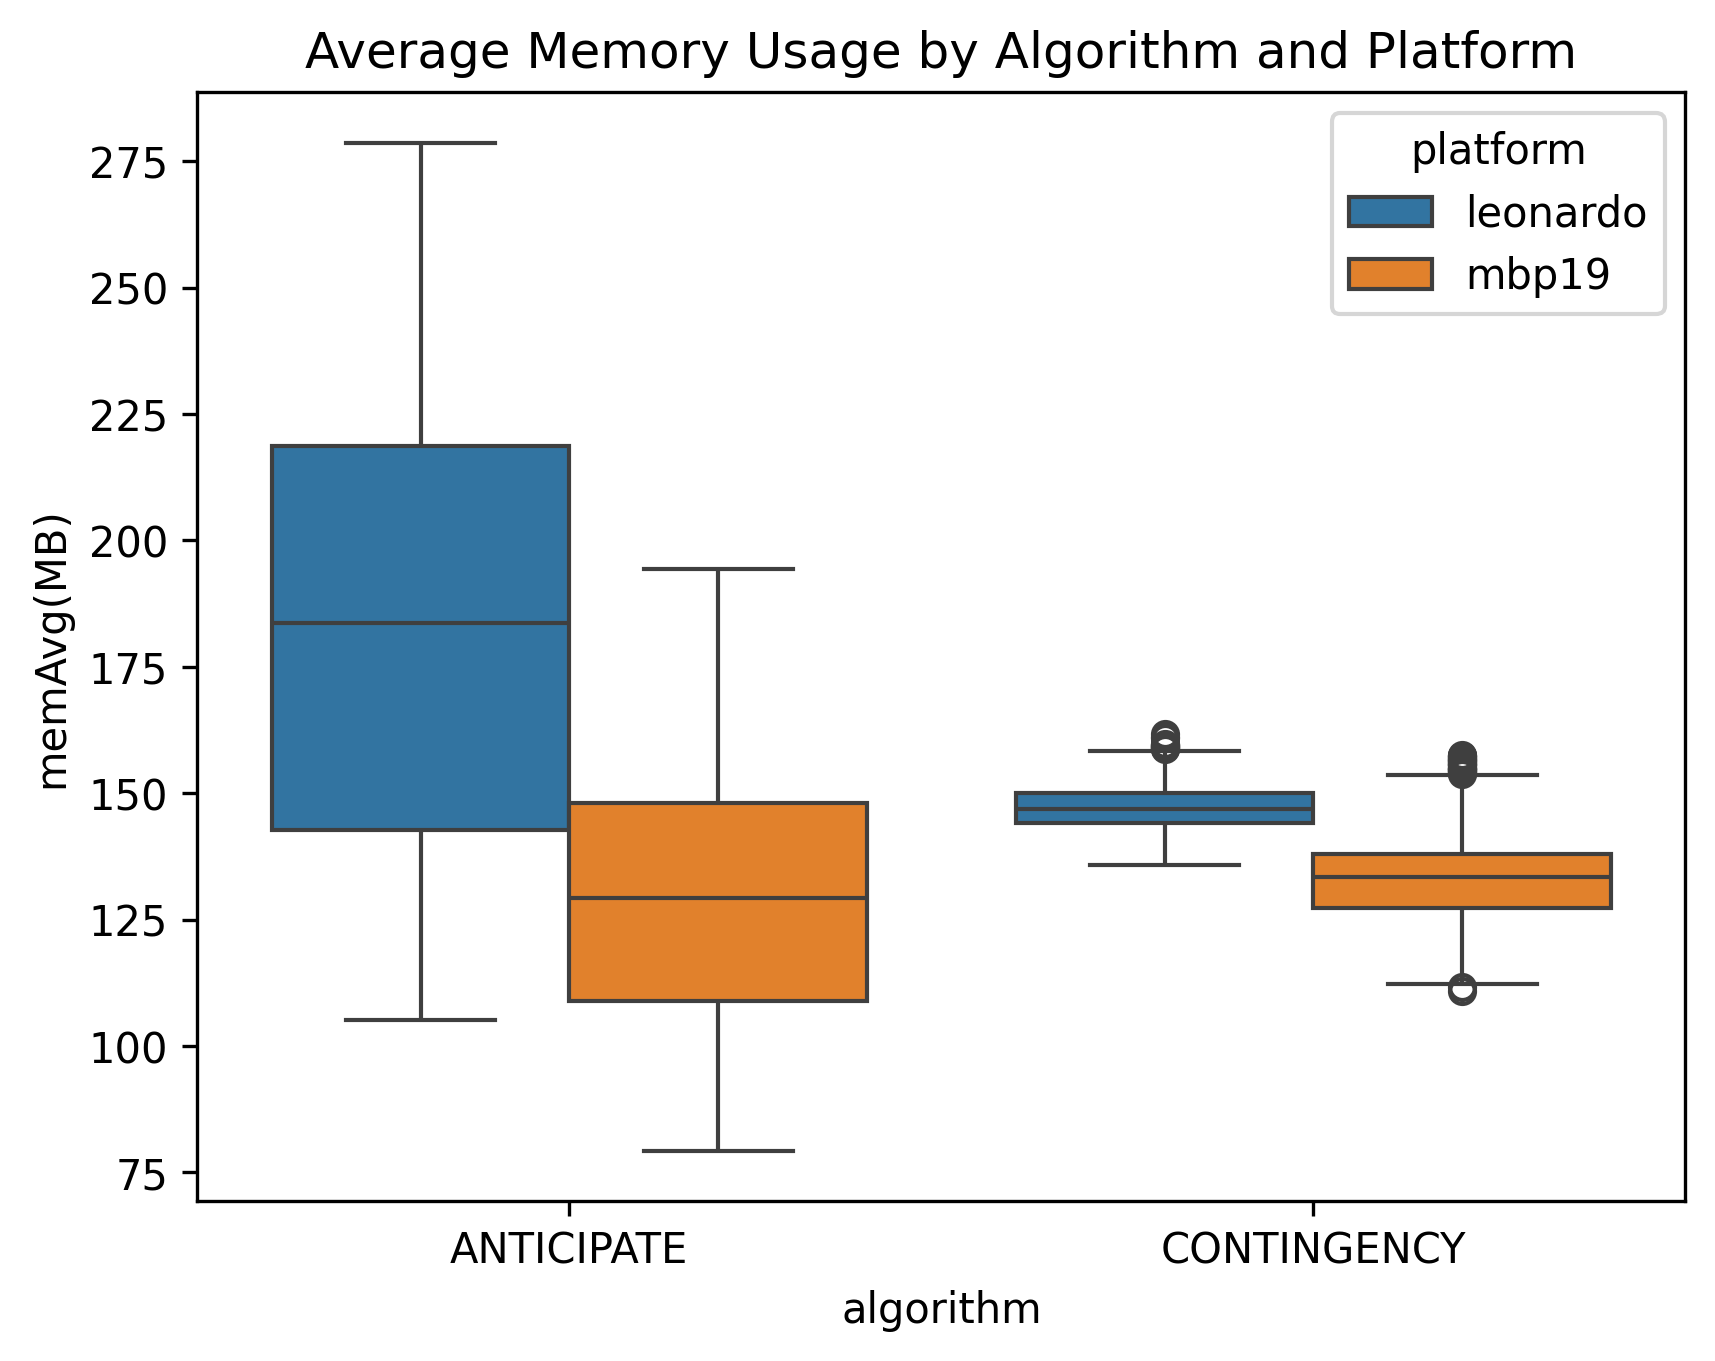
\includegraphics[width=\linewidth]{imgs/avg_mem_usage.png}
        \caption{Average memory usage}
        \label{fig:mem_usage_comparison}
    \end{subfigure}
    \begin{subfigure}[b]{0.4\linewidth}
        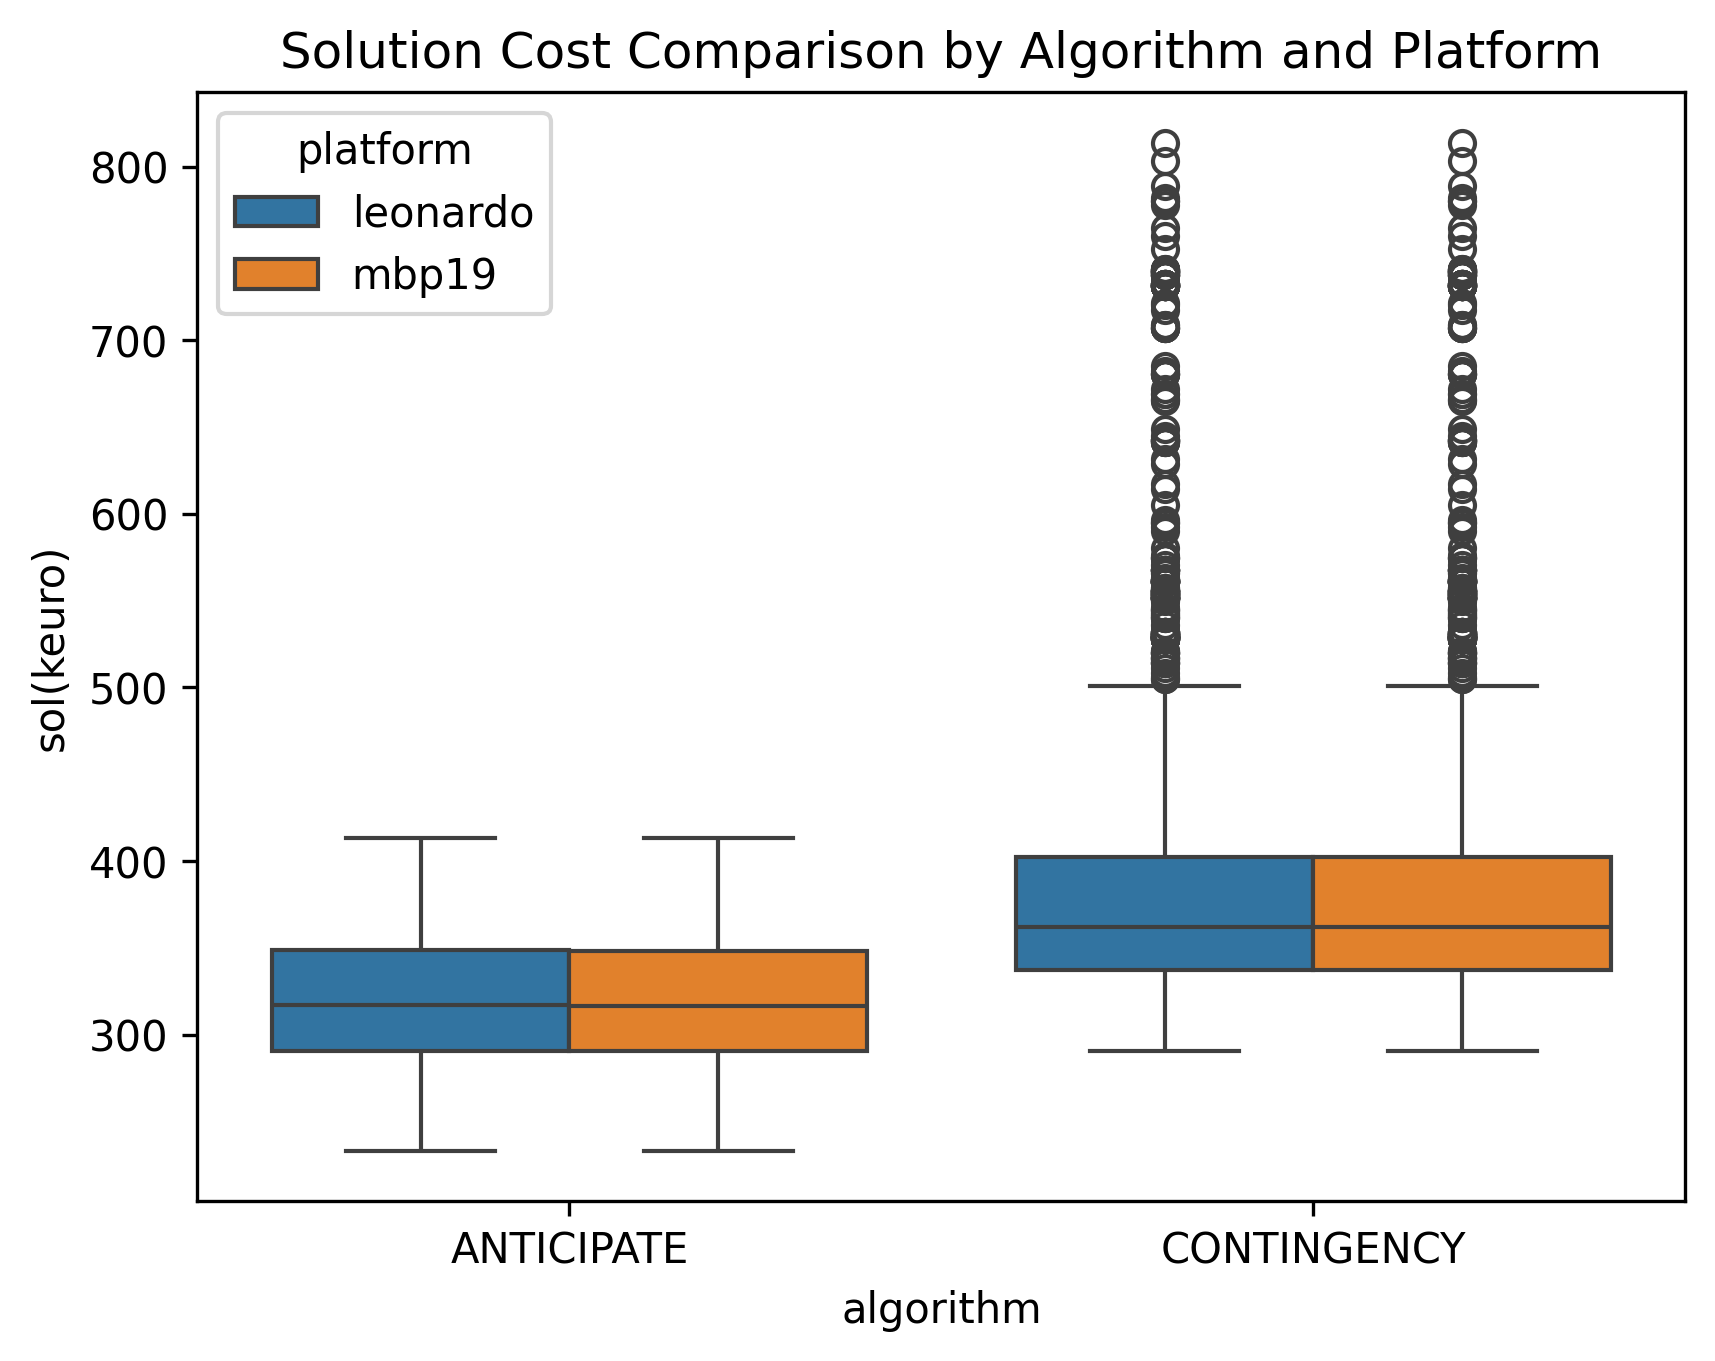
\includegraphics[width=\linewidth]{imgs/cost_comparison.png}
        \caption{Cost comparison}
        \label{fig:cost_comparison}
    \end{subfigure}
    \caption{Performance Comparison}
    \label{fig:comparison}
\end{figure}

\subsection{Min-Cut/Max-Flow Algorithms}

In this section, we analyze the performance and environmental impact of Min-Cut/Max-Flow algorithms and discuss the results obtained from tests performed using the HADA framework. 
These algorithms play a crucial role in various optimization problems, particularly in computer vision and network flow applications. Figure~\ref{fig:max_flow_emissions} presents an 
overview of the CO$_2$ emissions for the three Min-Cut/Max-Flow algorithms tested. It is evident that the vast majority of configurations emitted less than 0.001 kg of CO$_2$, 
similar to trends observed for the ANTICIPATE and CONTINGENCY algorithms.

\subsubsection{Carbon Emissions Analysis}

\begin{figure}[h!]
    \centering
    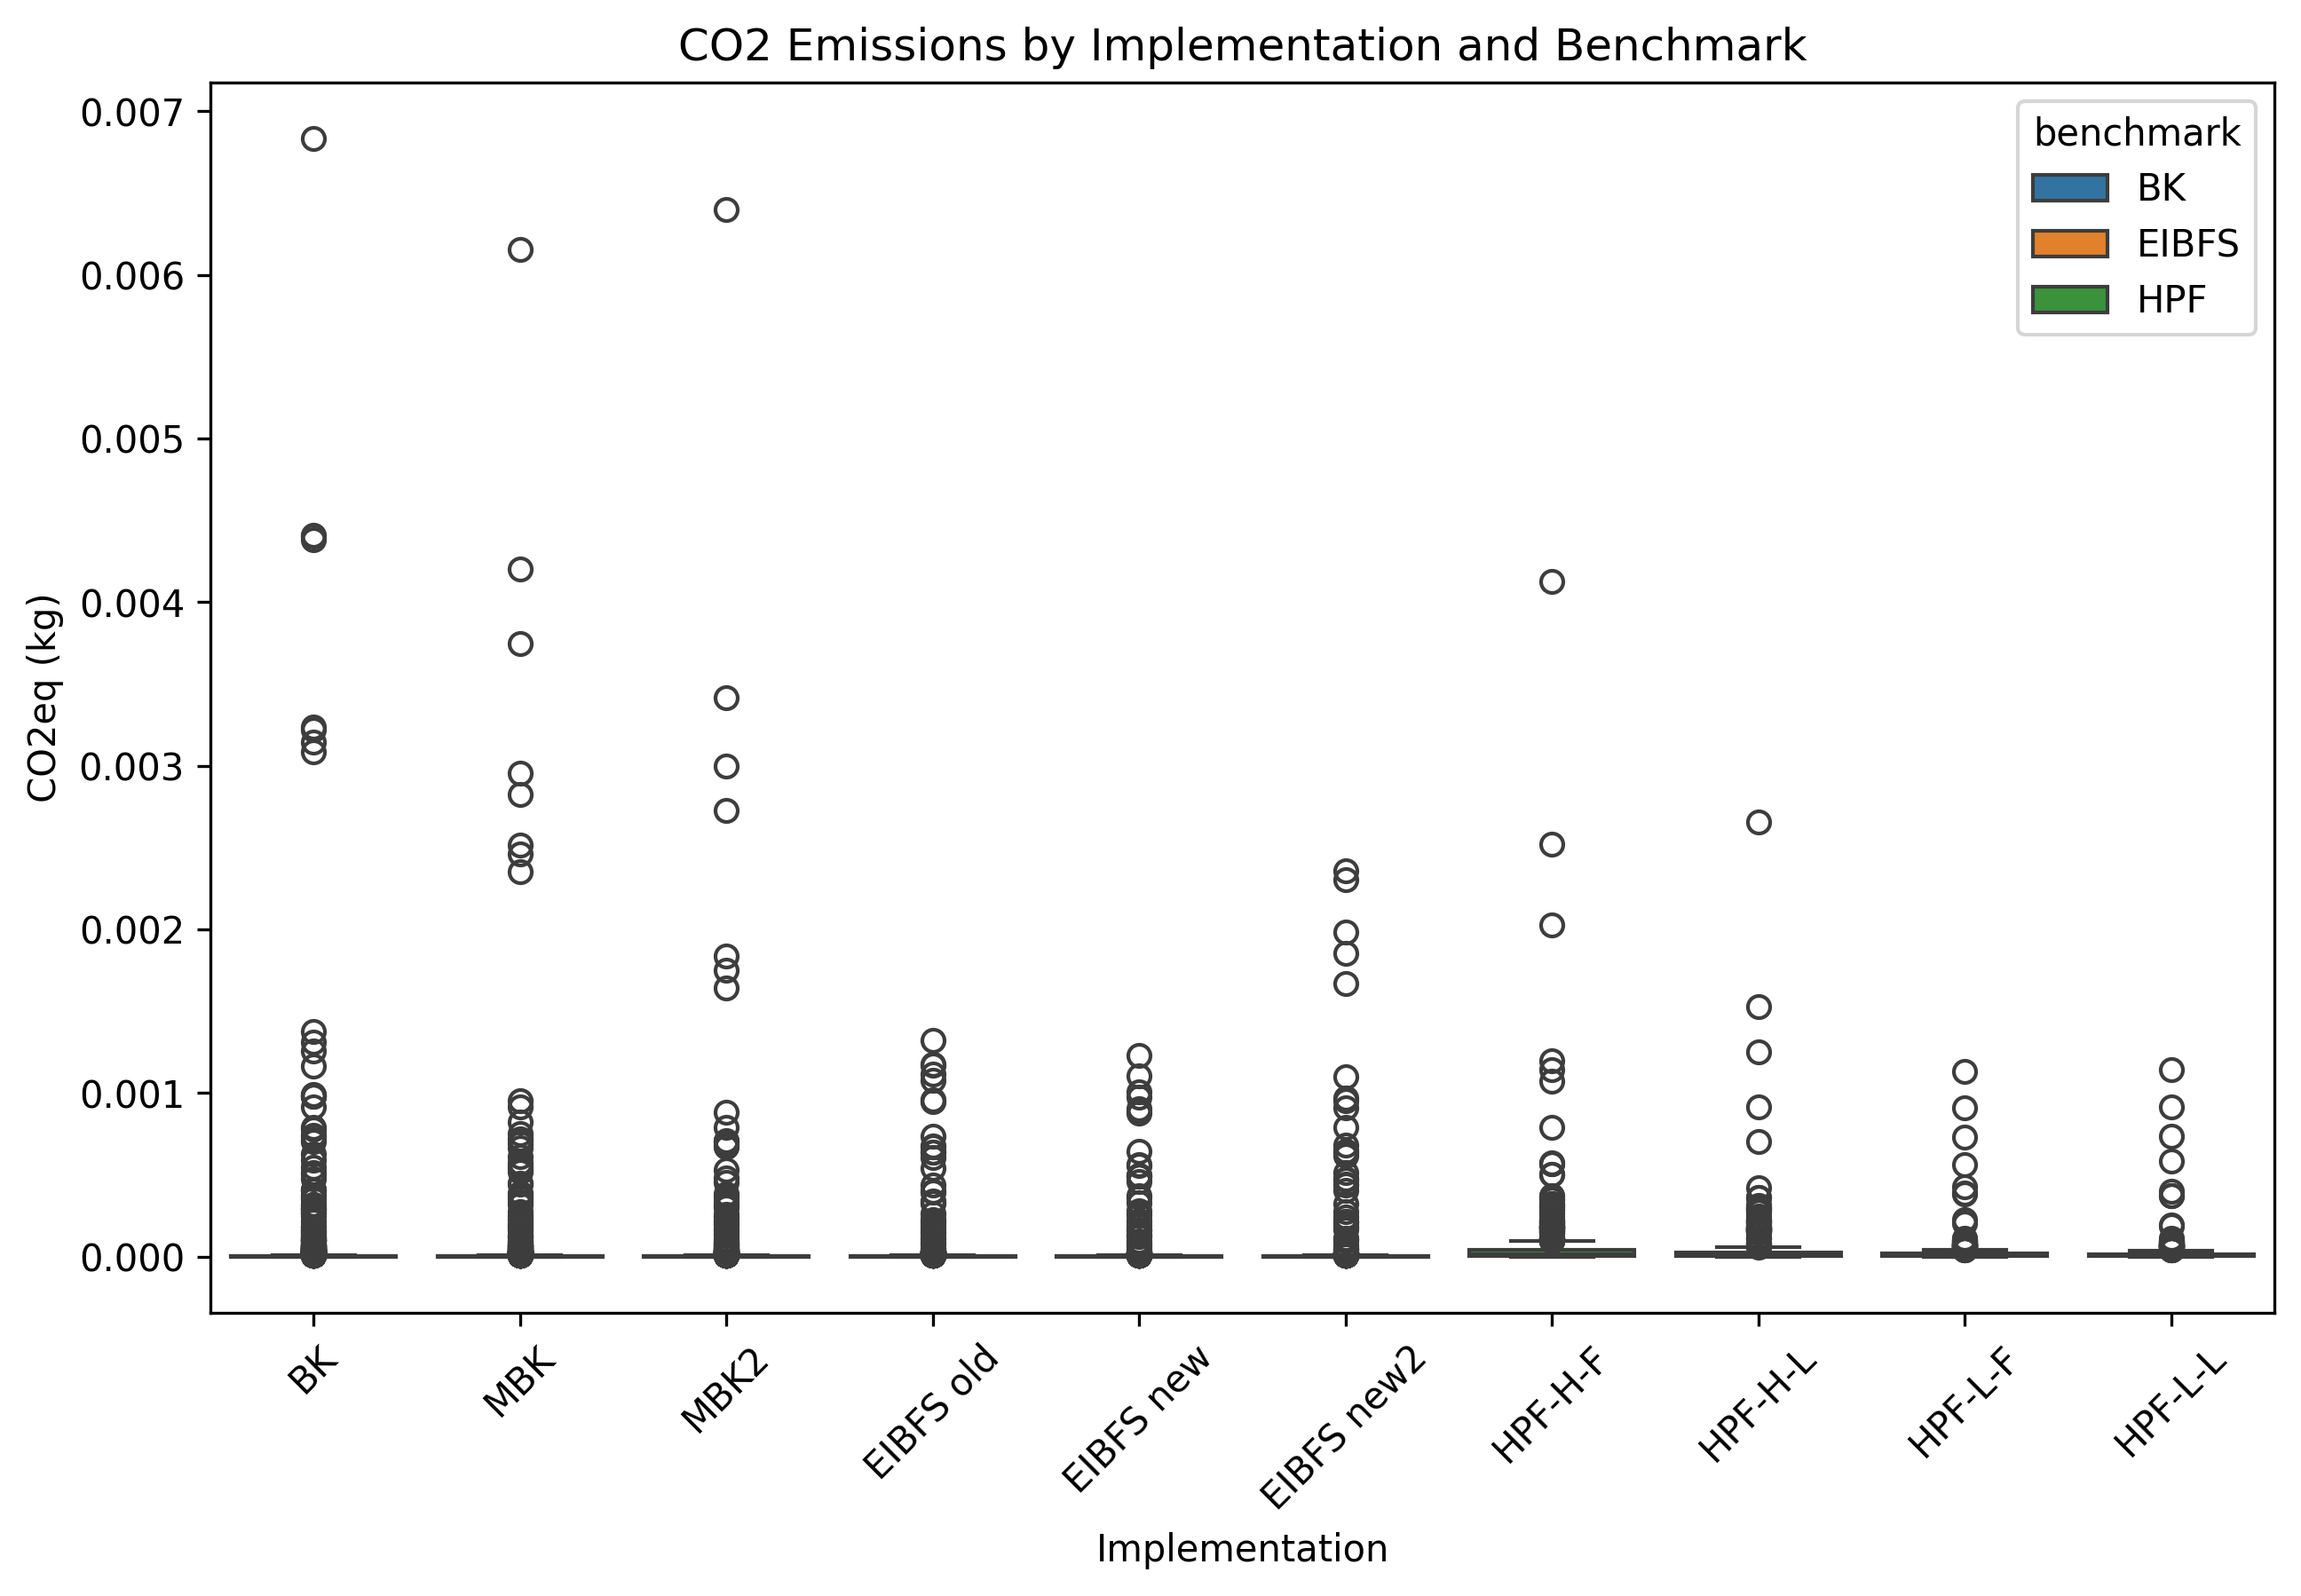
\includegraphics[width=0.8\textwidth]{imgs/max_flow_emissions.png}
    \caption{CO2 emissions for Min-Cut/Max-Flow algorithms}
    \label{fig:max_flow_emissions}
\end{figure}

By examining emissions data in Table \ref{tab:co2_benchmark}, we confirm that smaller architectures, such as \verb|pc| and \verb|mbp19|, tend to be more energy-efficient than the 
high-performance computing (HPC) system Leonardo. However, it is important to note that not all problem instances were executed on every platform due to constraints on memory 
availability and computational feasibility. 

\begin{table}[h]
    \centering
    \begin{tabular}{llccc}
        \hline
        \textbf{Algorithm} & \textbf{Platform} & \textbf{Mean} & \textbf{Min} & \textbf{Max} \\
        \hline
        \textbf{BK} & leonardo & $5.155456 \times 10^{-5}$ & $2.883260 \times 10^{-6}$ & 0.006184 \\
                    & pc       & $8.010042 \times 10^{-7}$ & $8.684843 \times 10^{-9}$ & 0.000145 \\
        \hline
        \textbf{EIBFS} & leonardo & $2.364746 \times 10^{-5}$ & $2.897591 \times 10^{-6}$ & 0.001861 \\
                       & pc       & $5.059142 \times 10^{-7}$ & $9.001983 \times 10^{-9}$ & 0.000027 \\
        \hline
        \textbf{HPF} & leonardo & $2.283886 \times 10^{-4}$ & $2.960032 \times 10^{-5}$ & 0.007584 \\
                     & mbp19    & $1.232039 \times 10^{-5}$ & $4.693739 \times 10^{-7}$ & 0.001145 \\
        \bottomrule
    \end{tabular}
    \caption{CO2e(kg) statistics for different algorithms and platforms.}
    \label{tab:co2_benchmark}
\end{table}

The discrepancy in emissions can largely be attributed to the scale of the problem instances executed on each platform. Due to the significantly larger memory available on Leonardo, 
the most demanding instances (with node counts reaching hundreds of millions) were exclusively executed on this HPC system. 

Additionally, some problem instances could not be solved by HPF implementations due to their reliance on negative capacity arcs. While BK and EIBFS supported such instances, HPF's 
current implementation does not, resulting in the exclusion of these cases from the dataset.

\subsubsection{Correlation Analysis}

To further understand the factors influencing emissions, Figures \ref{fig:bk_orr_mat}, \ref{fig:eibfs_corr_mat}, and \ref{fig:hpf_flow_corr_mat} present the correlation matrices for BK, 
EIBFS, and HPF, respectively. 

\begin{figure}[h!]
    \centering
    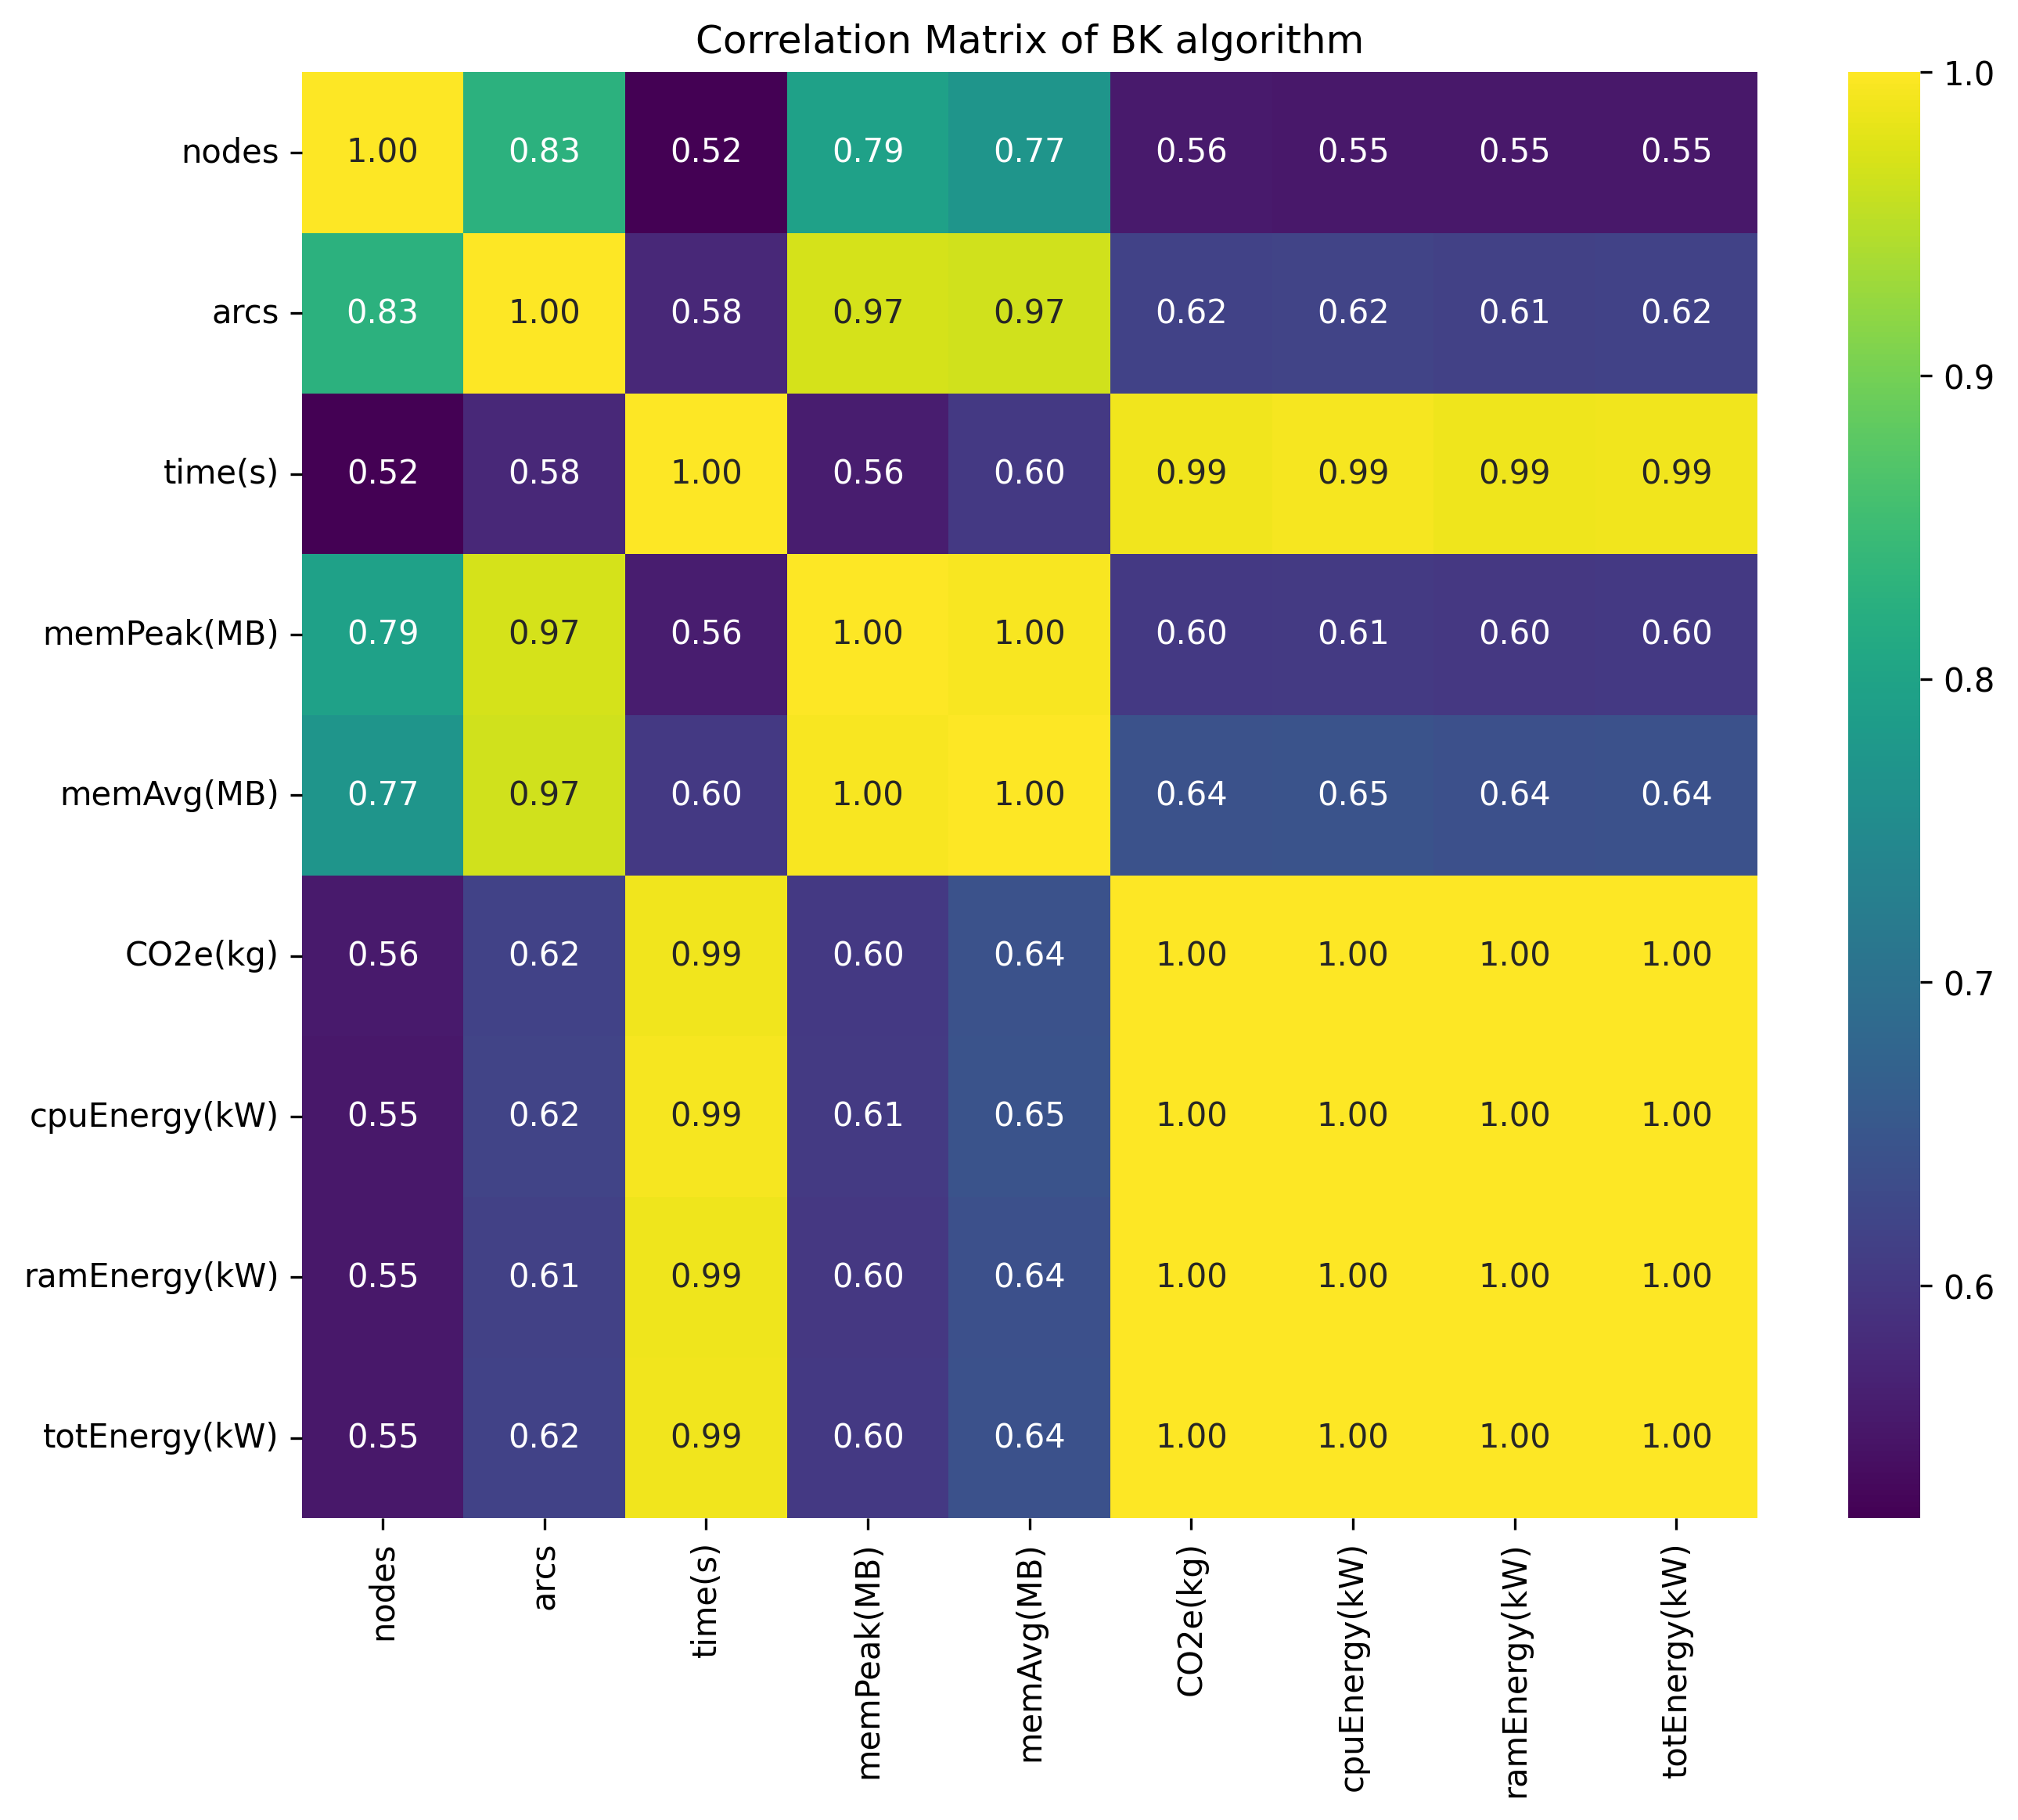
\includegraphics[width=0.8\textwidth]{imgs/bk_corr_mat.png}
    \caption{Correlation matrix for BK}
    \label{fig:bk_orr_mat}
\end{figure}

\begin{figure}[h!]
    \centering
    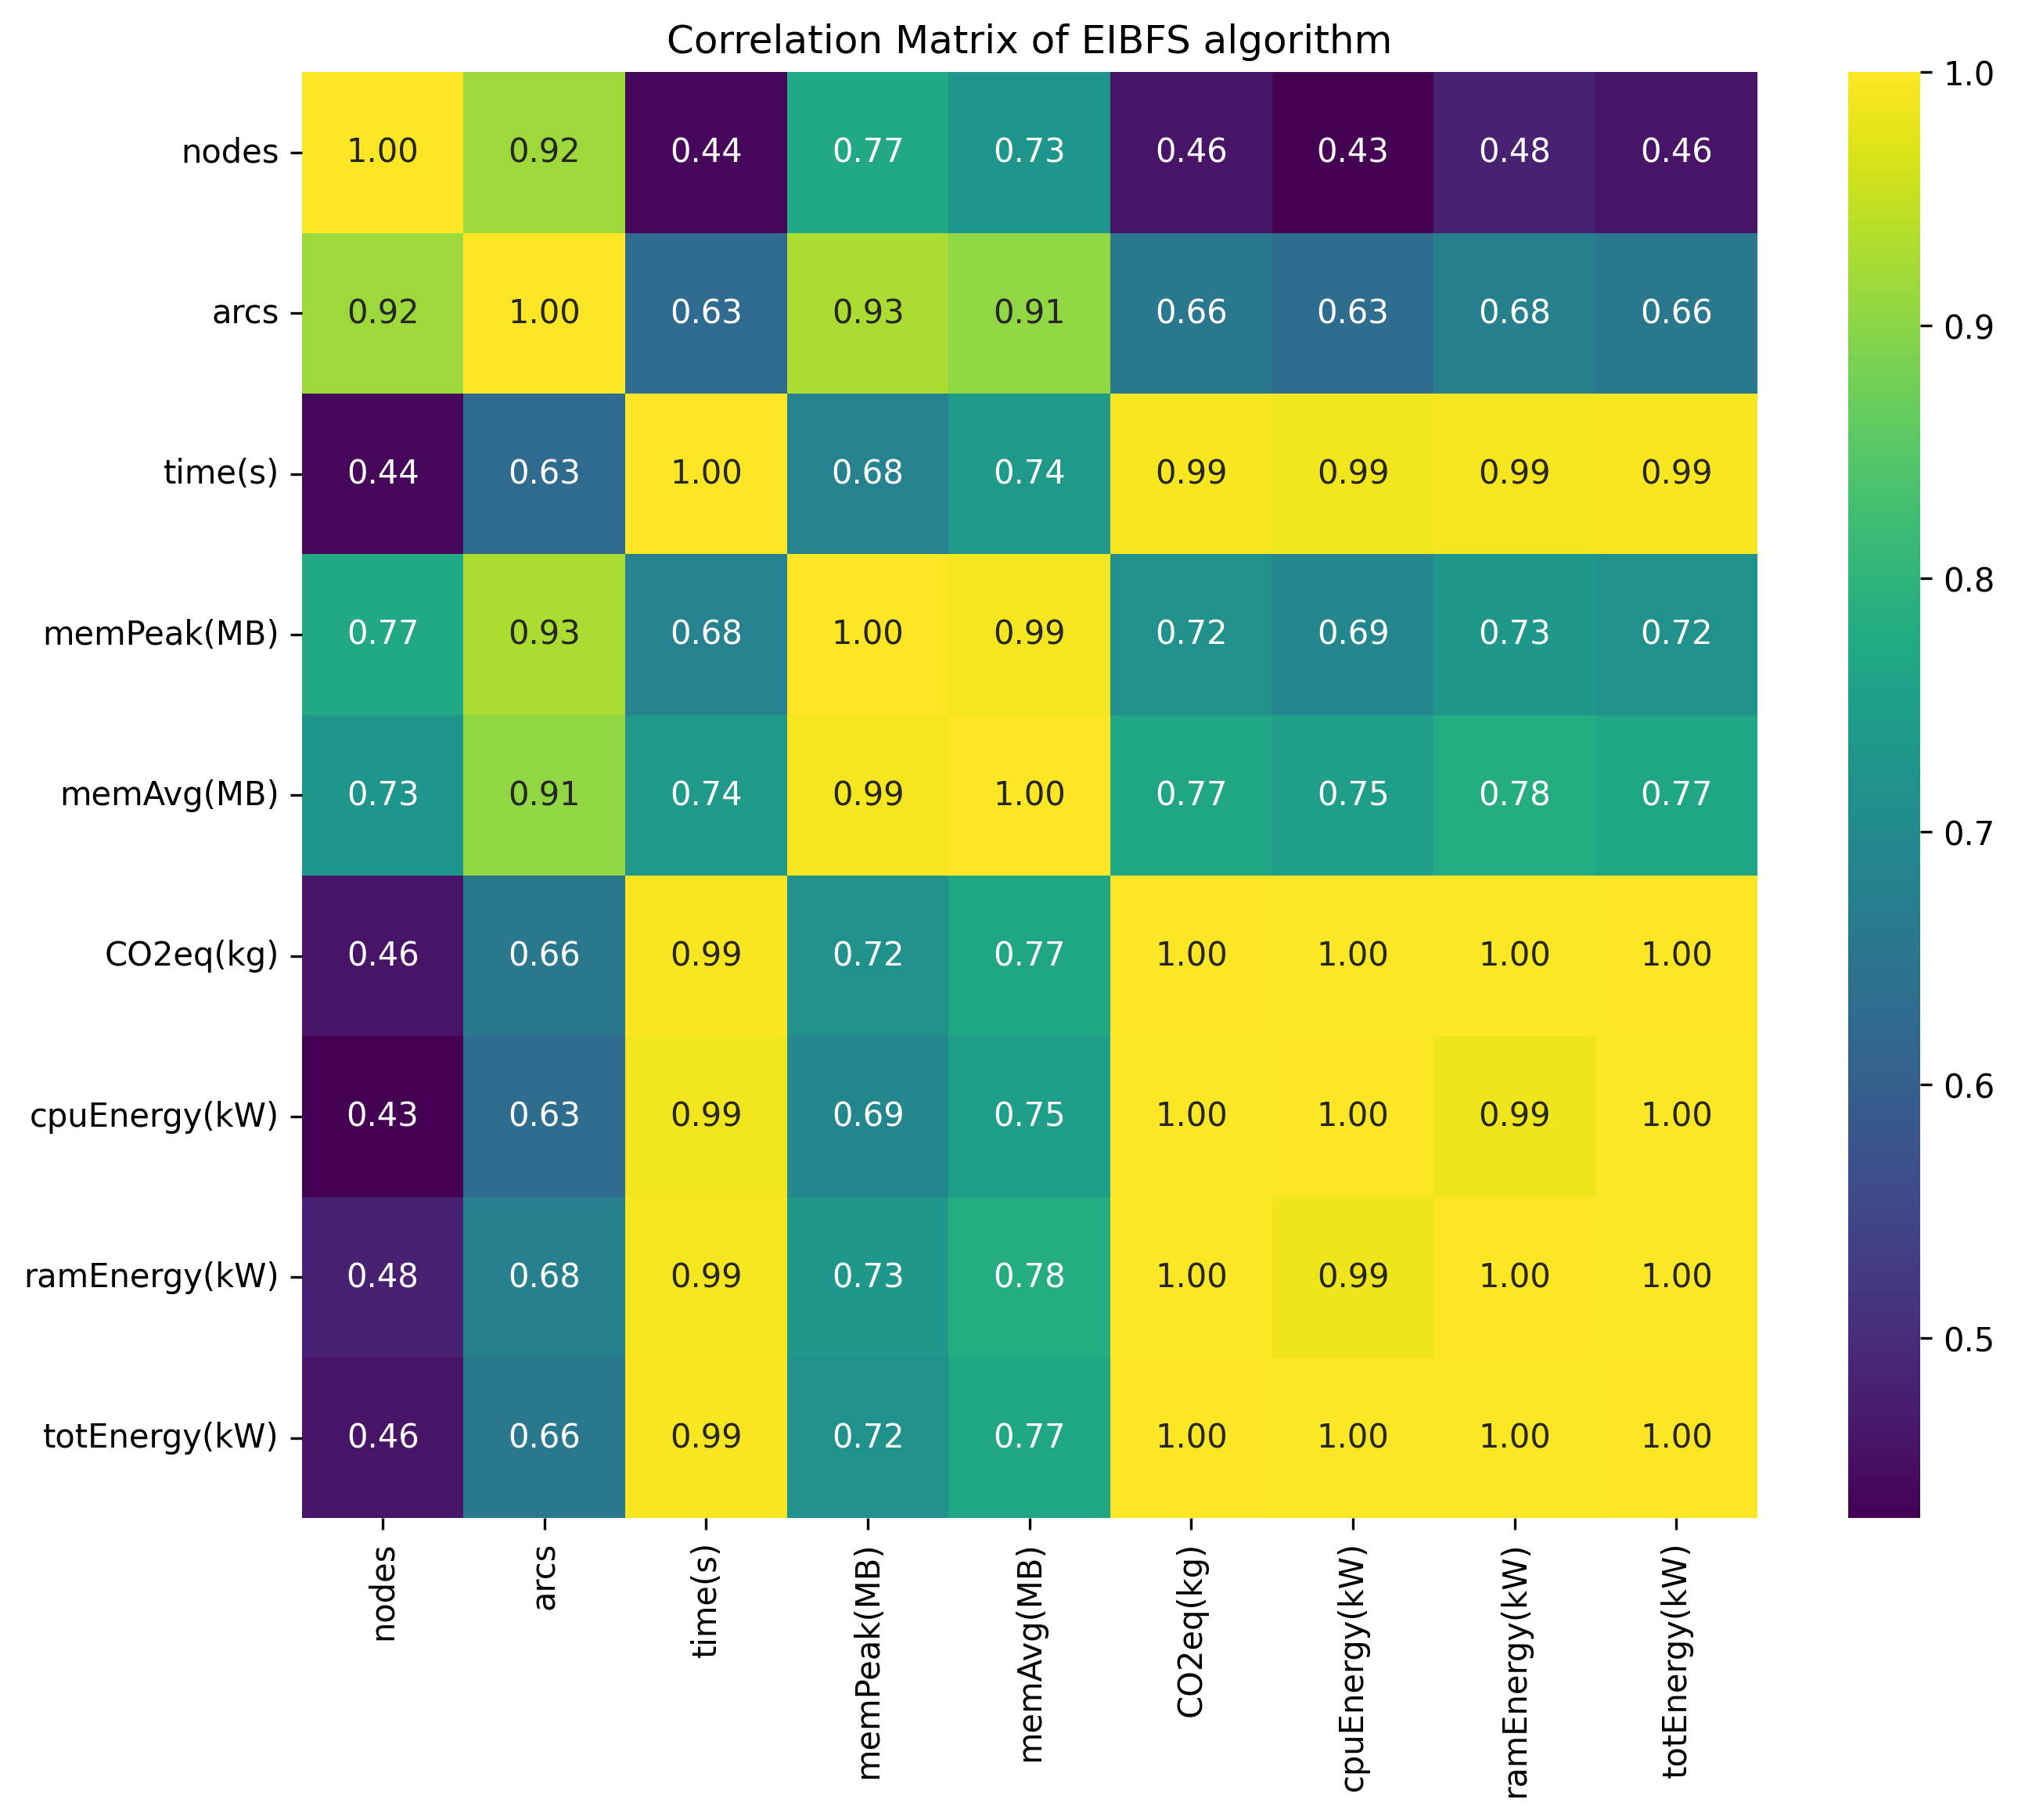
\includegraphics[width=0.8\textwidth]{imgs/eibfs_corr_mat.png}
    \caption{Correlation matrix for EIBFS}
    \label{fig:eibfs_corr_mat}
\end{figure}


\begin{figure}[h!]
    \centering
    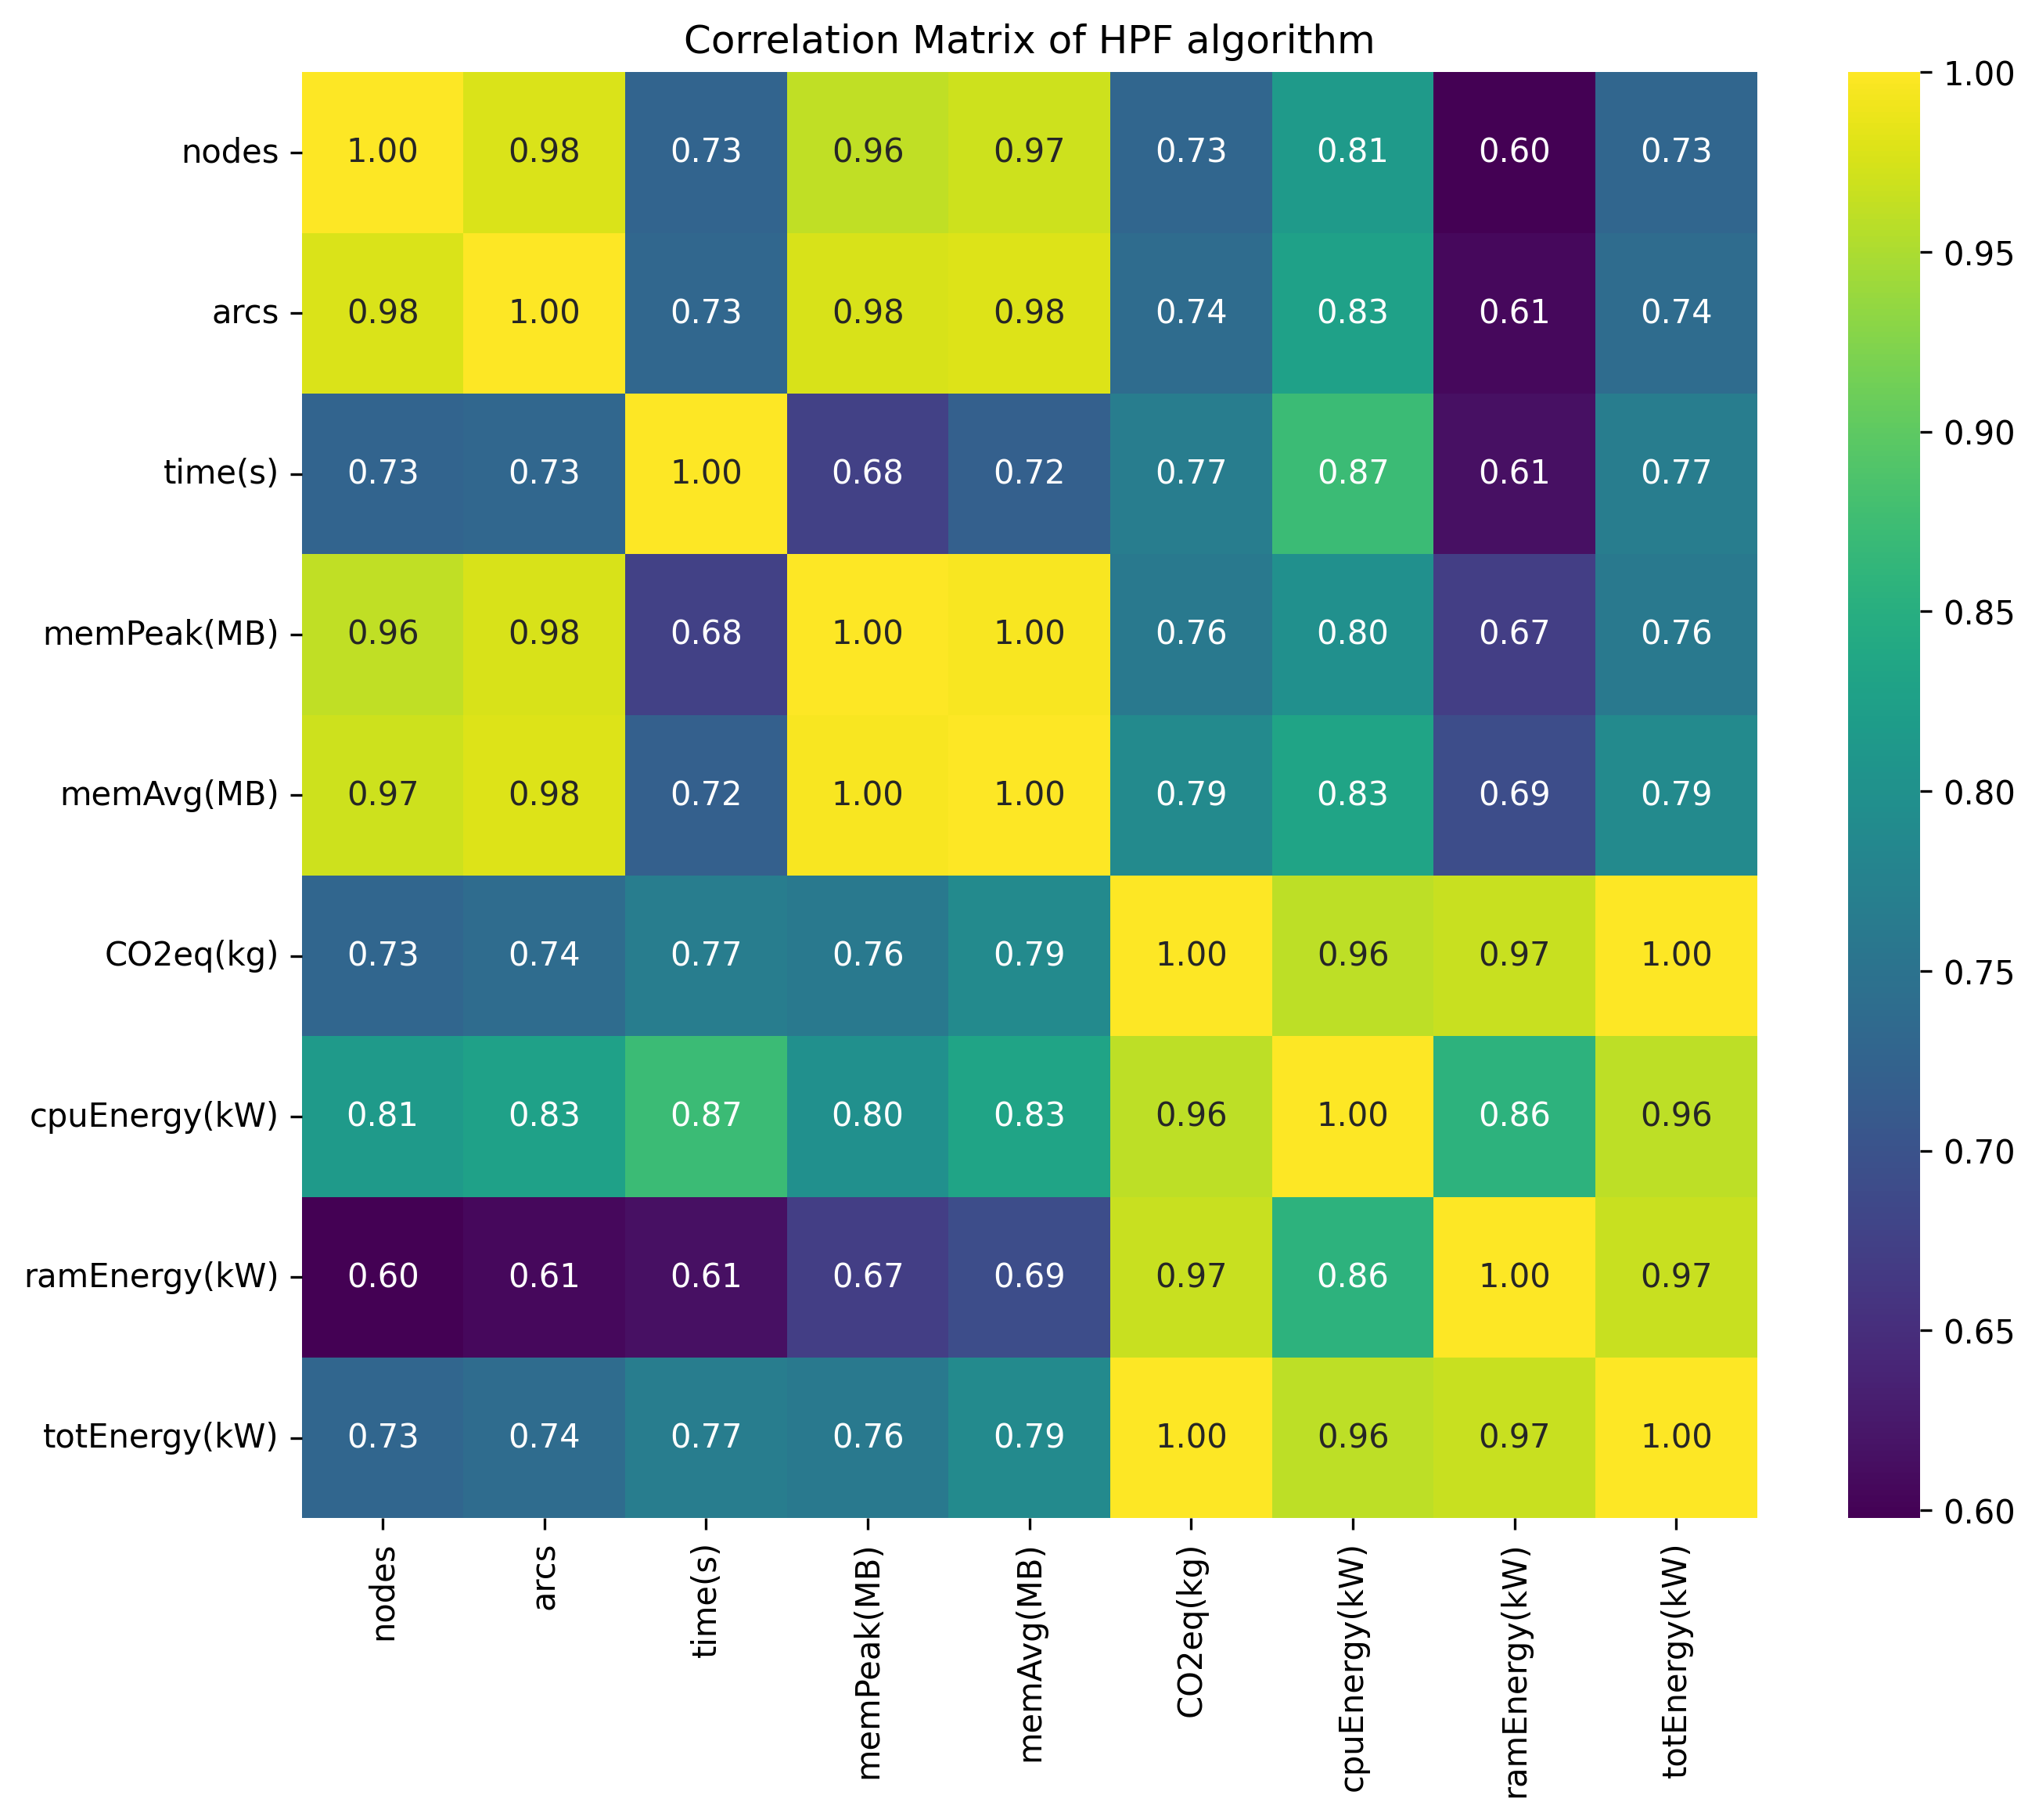
\includegraphics[width=0.8\textwidth]{imgs/hpf_corr_mat.png}
    \caption{Correlation matrix for BK}
    \label{fig:hpf_flow_corr_mat}
\end{figure}

For both BK and EIBFS, runtime exhibits the strongest correlation with CO$_2$ emissions. In Figure~\ref{fig:bk_orr_mat}, we observe that execution time has a correlation of approximately
$0.99$ with energy consumption and emissions, indicating that the longer an algorithm runs, the more energy it consumes, which directly translates into higher emissions. This trend 
is similarly observed in EIBFS (\ref{fig:eibfs_corr_mat}), reinforcing that for these algorithms, minimizing runtime is the most effective way to reduce emissions. Given this insight, 
we will assess how BK and EIBFS behave when constraints on runtime are introduced, particularly when minimizing CO$_2$ emissions.

HPF, on the other hand, demonstrates a slightly different behavior. From Figure~\ref{fig:hpf_flow_corr_mat}, we can see that the strongest correlation with CO$_2$ emissions is memory usage, 
specifically peak memory usage (memPeak) and average memory usage (memAvg), both exceeding 0.93. This suggests that rather than runtime alone, memory allocation plays a significant 
role in determining the carbon footprint of HPF. For this reason, in the experiments on HPF we impose constraints on peak memory usage rather than runtime.

\subsubsection{Performance Evaluation of Min-Cut/Max-Flow Algorithms with HADA}

In this section, we present the experimental results of optimizing the execution of Min-Cut/Max-Flow algorithms using HADA. The key objective was to evaluate the impact of different
hardware platforms (PC, mbp19, and Leonardo) on execution time, CO$_2$ emissions, and memory usage.

\paragraph{Optimization for CO$_2$ Emissions Minimization}

Tables \ref{tab:bk_results}, \ref{tab:eibfs_results}, and \ref{tab:hpf_results} summarize the results obtained when minimizing CO$_2$ emissions. Across all three algorithms, we observe
a strong preference for smaller-scale hardware platforms, with PC and mbp19 being consistently selected over Leonardo.

\begin{table}[h!]
    \centering
    \begin{tabular}{|ccc|cccc|}
        \hline
        \multicolumn{3}{|c|}{Inputs \& Bound} & \multicolumn{4}{c|}{Solution} \\
        \hline
        Nodes & Arcs & time(s) & Impl. & HW & CO2e & time(s) \\
        \hline
        40 & 400 & $0.1$ & MBK2 & pc & $4.38 \times 10^{-7}$ & $3.81 \times 10^{-5}$ \\
        120 & 2k & $0.1$ & MBK2 & pc & $4.40 \times 10^{-7}$ & $5.10 \times 10^{-5}$ \\
        1k & 5k & $0.1$ & MBK & pc & $4.40 \times 10^{-7}$ & $4.09 \times 10^{-4}$ \\
        10k & 62k & $0.1$ & BK & pc & $4.40 \times 10^{-7}$ & $2.63 \times 10^{-3}$ \\
        44k & 784k & $5$ & MBK2 & pc & $6.46 \times 10^{-6}$ & $1.39$ \\
        185k & 5M & $5$ & MBK2 & pc & $2.16 \times 10^{-6}$ & $0.28$ \\
        18M & 93M & $10$ & MBK2 & pc & $4.69 \times 10^{-5}$& $9.79$ \\
        \hline
    \end{tabular}
    \caption{Experimental results for the BK algorithm, with constraints on the runtime}
    \label{tab:bk_results}
\end{table}

\begin{table}[h!]
    \centering
    \begin{tabular}{|ccc|cccc|}
        \hline
        \multicolumn{3}{|c|}{Inputs \& Bound} & \multicolumn{4}{c|}{Solution} \\
        \hline
        Nodes & Arcs & time(s) & Impl. & HW & CO2e & time(s) \\
        \hline
        40 & 400 & $0.1$ & EIBFS new & pc & $4.37 \times 10^{-7}$ & $3.75 \times 10^{-5}$ \\
        120 & 2k & $0.1$ & EIBFS new & pc & $4.40 \times 10^{-7}$ & $1.80 \times 10^{-4}$ \\
        1k & 5k & $0.1$ & EIBFS new & pc & $4.40 \times 10^{-7}$ & $2.03 \times 10^{-4}$ \\
        10k & 62k & $0.1$ & EIBFS old & pc & $4.40 \times 10^{-7}$ & $2.89 \times 10^{-3}$ \\
        44k & 784k & $0.5$ & EIBFS new & pc & $8.7 \times 10^{-7}$ & $0.27$ \\
        185k & 5M & $0.5$ & EIBFS new2 & pc & $1.30 \times 10^{-6}$ & $0.12$ \\
        3M & 23M & $5$ & EIBFS new & pc & $1.98 \times 10^{-5}$& $3.51$ \\
        \hline
    \end{tabular}
    \caption{Experimental results for the EIBFS algorithm, minimising CO$_2$ emissions with constraints on the runtime}
    \label{tab:eibfs_results}
\end{table}

\begin{table}[h!]
    \centering
    \begin{tabular}{|ccc|cccc|}
        \hline
        \multicolumn{3}{|c|}{Inputs \& Bound} & \multicolumn{4}{c|}{Solution} \\
        \hline
        Nodes & Arcs & Mem(MB) & Impl. & HW & CO2e & Mem(MB) \\
        \hline
        2.5k & 50k & $10$ & HPF-H-F & mbp19 & $2.11 \times 10^{-6}$ & $0.48$ \\
        10k & 75k & $10$ & HPF-H-F & mbp19 & $4.91 \times 10^{-7}$ & $0.46$ \\
        100k & 300k & $100$ & HPF-L-L & mbp19 & $9.56 \times 10^{-7}$ & $15.46$ \\
        300k & 500k & $100$ & HPF-L-L & mbp19 & $1.46 \times 10^{-6}$ & $35.45$ \\
        1M & 5M & $100$ & none & none & none & none \\
        1M & 5M & $400$ & HPF-L-L & mpb19 & $8.25 \times 10^{-6}$ & $390.83$ \\
        10M & 25M & none & none & none & none & none \\
        10M & 25M & $3000$ & HPF-H-L & mbp19 & $6.85 \times 10^{-5}$ & $2122.97$ \\
        125M & 300M & $4000$ & HPF-L-F & mbp19 & $9.08 \times 10^{-3}$ & $3785.29$ \\
        \hline
    \end{tabular}
    \caption{Experimental results for the HPF algorithm, with constraints on peak memory consumption}
    \label{tab:hpf_results}
\end{table}

Similar trends were observed for EIBFS and HPF, as shown in Tables \ref{tab:eibfs_results} and \ref{tab:hpf_results}. When CO$_2$ emissions were minimized, the computationally
lighter hardware architectures were consistently preferred. 

\paragraph{Optimization for Runtime Minimization}

To explore whether HPC would provide a significant advantage in execution time, we re-ran HADA optimization while minimizing runtime instead of emissions. The results for BK, EIBFS, 
and HPF are presented in Tables \ref{tab:bk_results_time}, \ref{tab:eibfs_results_runtime}, and \ref{tab:hpf_results_runtime}.

\begin{table}[h!]
    \centering
    \begin{tabular}{|ccc|cccc|}
        \hline
        \multicolumn{3}{|c|}{Inputs \& Bound} & \multicolumn{4}{c|}{Solution} \\
        \hline
        Nodes & Arcs & CO2e(kg) & Impl. & HW & CO2e & time(s) \\
        \hline
        40 & 400 & $0.001$ & MBK2 & pc & $4.38 \times 10^{-7}$ & $3.81 \times 10^{-5}$ \\
        120 & 2k & $0.001$ & MBK2 & pc & $4.40 \times 10^{-7}$ & $5.10 \times 10^{-5}$ \\
        1k & 5k & $0.001$ & MBK & leonardo & $4.40 \times 10^{-7}$ & $1.10 \times 10^{-4}$ \\
        10k & 62k & $0.001$ & MBK & leonardo & $4.40 \times 10^{-7}$ & $2.32 \times 10^{-3}$ \\
        16k & 111k & $0.1$ & MBK & leonardo & $4.44 \times 10^{-5}$ & $1.37$ \\
        44k & 784k & $0.1$ & MBK2 & leonardo & $2.63 \times 10^{-6}$ & $0.88$ \\
        185k & 5M & $0.1$ & MBK2 & pc & $2.16 \times 10^{-6}$ & $0.28$ \\
        3M & 23M & $0.1$ & MBK2 & leonardo & $9.53 \times 10^{-5}$& $2.67$ \\
        \hline
    \end{tabular}
    \caption{Experimental results for the BK algorithm, minimizing runtime and bounding CO$_2$ emissions}
    \label{tab:bk_results_time}
\end{table}

For smaller problem instances, we see that PC and mbp19 remain preferable (see \ref{tab:bk_results_time}). However, in some cases involving larger problem sizes (e.g., 16k nodes, 111k arcs), HADA selects Leonardo. 
Despite this, the improvement in runtime is not substantial, with the execution time on PC being approximately $4.09 \times 10^{-4}$ seconds compared to $1.10 \times 10^{-4}$ 
seconds on Leonardo.

\begin{table}[h!]
    \centering
    \begin{tabular}{|ccc|cccc|}
        \hline
        \multicolumn{3}{|c|}{Inputs \& Bound} & \multicolumn{4}{c|}{Solution} \\
        \hline
        Nodes & Arcs & CO2(kg) & Impl. & HW & CO2e & time(s) \\
        \hline
        40 & 400 & $0.1$ & EIBFS new2 & leonardo & $3.01 \times 10^{-6}$ & $1.37 \times 10^{-5}$ \\
        120 & 2k & $0.1$ & EIBFS new2 & leonardo & $3.01 \times 10^{-6}$ & $7.22 \times 10^{-5}$ \\
        1k & 5k & $0.1$ & EIBFS new2 & leonardo & $4.40 \times 10^{-6}$ & $7.23 \times 10^{-4}$ \\
        10k & 62k & $0.1$ & EIBFS new2 & leonardo & $4.40 \times 10^{-6}$ & $1.72 \times 10^{-3}$ \\
        44k & 784k & $0.1$ & EIBFS new2 & leonardo & $9.27 \times 10^{-6}$ & $0.02$ \\
        185k & 5M & $0.1$ & EIBFS new2 & leonardo & $8.80 \times 10^{-6}$ & $0.09$ \\
        3M & 23M & $0.1$ & EIBFS new & leonardo & $8.24 \times 10^{-5}$& $2.19$ \\
        \hline
    \end{tabular}
    \caption{Experimental results for the EIBFS algorithm, minimising runtime, with bounds on CO$_2$ emissions}
    \label{tab:eibfs_results_runtime}
\end{table}

For EIBFS (see \ref{tab:eibfs_results_runtime}), results still confirm this trend even if in these case we have more configurations with leonardo.

\begin{table}[h!]
    \centering
    \begin{tabular}{|ccc|cccc|}
        \hline
        \multicolumn{3}{|c|}{Inputs \& Bound} & \multicolumn{4}{c|}{Solution} \\
        \hline
        Nodes & Arcs & CO2e(kg) & Impl. & HW & CO2e & time(s) \\
        \hline
        2.5k & 50k & $0.1$ & HPF-H-F & leonardo & $3.58 \times 10^{-6}$ & 0.001 \\
        10k & 75k & $0.1$ & HPF-H-L & leonardo & $2.98 \times 10^{-6}$ & 0.002 \\
        16k & 111k & $0.1$ & HPF-H-F & leonardo & $1.02 \times 10^{-3}$ & 11.648 \\
        15k & 200k & $0.1$ & HPF-H-F & leonardo & $1.55 \times 10^{-3}$ & 2.214 \\
        134k & 921k & $0.1$ & HPF-L-F & leonardo & $1.46 \times 10^{-6}$ & 9.278 \\
        1M & 5M & $0.1$ & HPF-L-L & mpb19 & $8.25 \times 10^{-6}$ & 0.062 \\
        10M & 25M & $3000$ & HPF-H-L & mbp19 & $6.85 \times 10^{-5}$ & 5.31 \\
        125M & 300M & $4000$ & HPF-L-F & mbp19 & $9.08 \times 10^{-3}$ & 27.74 \\
        \hline
    \end{tabular}
    \caption{Experimental results for the EIBFS algorithm}
    \label{tab:hpf_results_runtime}
\end{table}

For HPF, similar results hold, with mbp19 being preferred for smaller instances, while Leonardo is selected for medium-sized problems.

\paragraph{Discussion: Why Does HPC Not Show a Significant Runtime Advantage?}

From the results obtained, we observe that even when optimizing for runtime, HADA often does not favor HPC. Several factors contribute to this:

\begin{itemize}
    \item Sequential Algorithm Implementations: the versions of BK, EIBFS, and HPF tested in this study were single-threaded, meaning they do not take advantage of parallel 
    processing capabilities offered by HPC clusters. As highlighted by Jensen et al. \cite{Jensen2023Maxflow}, specialized parallel implementations of max-flow algorithms exist, 
    and these would likely benefit more from HPC architectures. Then, neither the Min-Cut/Max-Flow algorithms nor the energy management algorithms rely on the use of GPUs, 
    which tipycally can create a large speedup. So, again, we did not have the settings to exploit the full potential of an HPC cluster.
    \item Computational Overhead in HPC systems: HPC environments like Leonardo introduce additional computational overhead due to factors such as job scheduling, data transfer, 
    and process management. For small and medium-sized instances, this overhead can negate the potential runtime benefits, leading to comparable or even worse performance compared 
    to commodity hardware. %TODO: incorporate observations 
\end{itemize}

\chapter{HADA-as-a-Service}

\section{HADA Web Application}

The HADA framework, which was used to conduct the experiments in this study, has also been implemented as a web application. This implementation provides a user-friendly interface 
for defining optimization problems, specifying constraints, and selecting the appropriate computational setup. The interface of the HADA web service application is depicted in 
\ref{fig:hada_ui}.

\begin{figure}[h!]
    \centering
    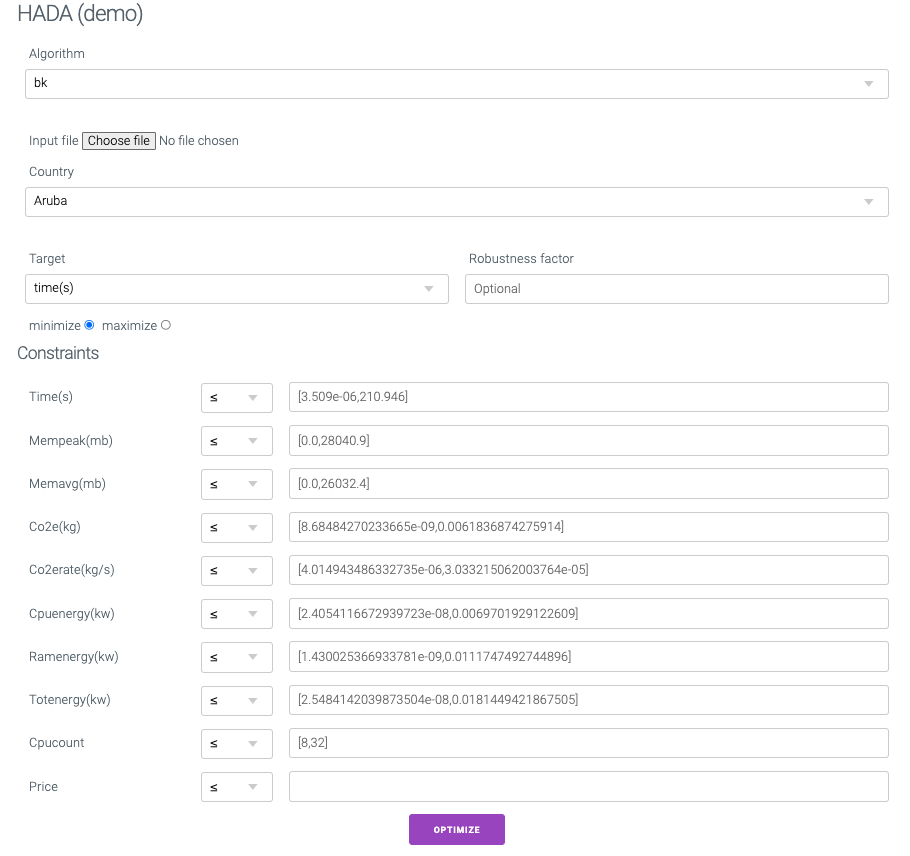
\includegraphics[width=\textwidth]{imgs/HADA-main-ui.png}
    \caption{The UI for the HADA web service application}
    \label{fig:hada_ui}
\end{figure}

The web interface is designed to simplify the optimization process by offering several key functionalities:
\begin{itemize}
    \item Algorithm Selection: A dropdown menu allows the user to select the target algorithm for optimization.
    \item Input File Uploader: For input-dependent algorithms, users can upload input datasets required for execution.
    \item Geographic Selection: The user can select the country where the computation will be performed. This is crucial as it affects the carbon emissions estimation based on region-specific Carbon Intensity values.
    \item Optimization Target: The user can specify which metric to optimize, such as execution time, energy consumption, or carbon emissions.
    \item Robustness Factor: An optional setting that allows to specify confidence level for the user defined constraints
    \item Constraint Specification: Users can define constraints on various performance metrics (e.g., execution time, memory usage, CO$_2$ emissions). Constraints can be defined as:
    \begin{itemize}
        \item $\leq$ (Upper bound) 
        \item $\geq$ (Lower bound)
        \item $=$ (Fixed value)
    \end{itemize} 
    \item The "Optimise" button, which launches the optimization process.
\end{itemize}

When the optimization starts, the HADA backend performs the following steps:
\begin{itemize}
    \item Model Checking: The system verifies if pre-trained models exist for the required combination of (Algorithm, Hardware, Target). If a model is unavailable, HADA trains a new one.
    \item Machine Learning Models: The ML models used are Decision Tree Regressors with a maximum depth of 10. These models were found to provide a good balance between prediction accuracy and computational complexity \cite{DEFILIPPO2022109199}.
    \item Integration with Optimization Engine: The trained ML models are incorporated into the optimization problem as constraints.
    \item Solving the Optimization Model: The mathematical model, including user-defined constraints, is passed to IBM CPLEX, which attempts to find an optimal solution.
\end{itemize}

An example of an optimization request sent through the HADA GUI is depicted in Figure~\ref{fig:hada_optimisation_req}.

\begin{figure}[h!]
    \centering
    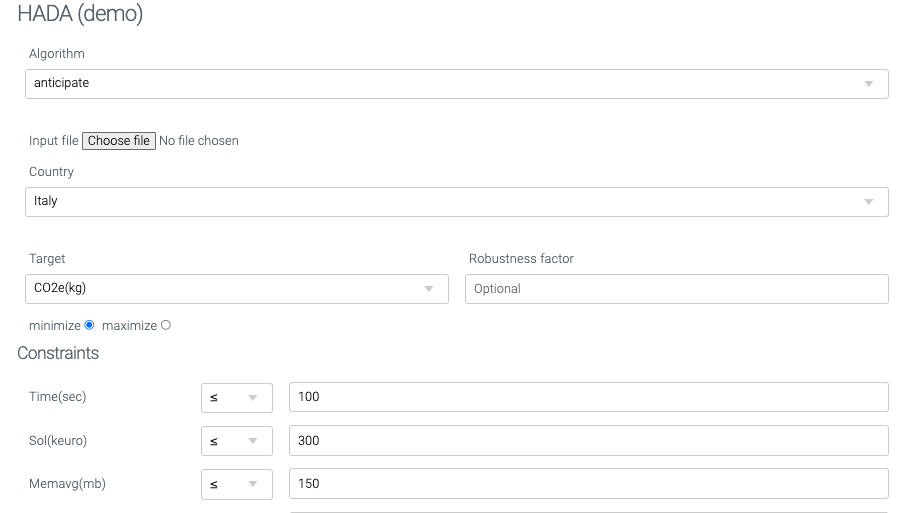
\includegraphics[width=\textwidth]{imgs/HADA-optimisation-req.png}
    \caption{Example of an optimisation request sent to HADA via the GUI}
    \label{fig:hada_optimisation_req}
\end{figure}

If a feasible solution is found, the HADA GUI displays the optimal configuration, including the selected hardware platform, algorithm hyperparameters, and the estimated performance metrics, as shown in Figure~\ref{fig:hada_solution}.

\begin{figure}[h!]
    \centering
    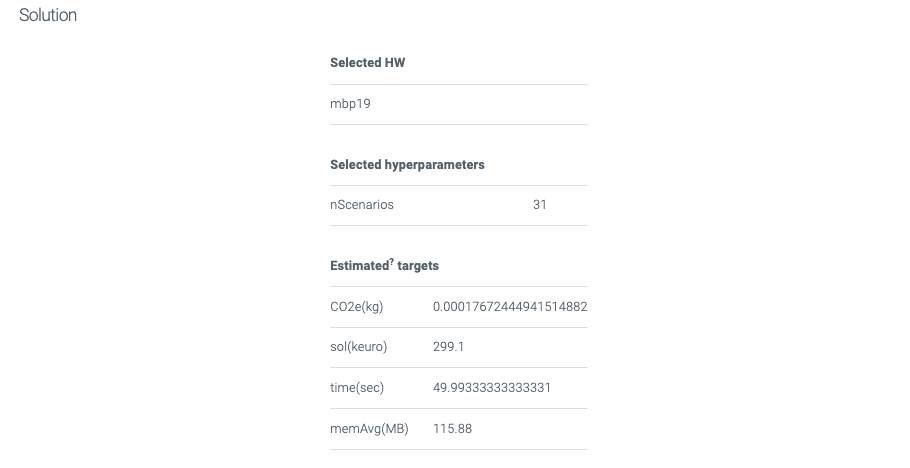
\includegraphics[width=\textwidth]{imgs/hada-solution-italy.png}
    \caption{The solution provided for the above example in Figure~\ref{fig:hada_optimisation_req}}
    \label{fig:hada_solution}
\end{figure}

One of the key aspects of this work was to extend HADA account for geographical variations in Carbon Intensity when computing emissions. To demonstrate this, we perform the same 
optimization request but change the execution location. For example, Figure~\ref{fig:hada_solution_turkmenistan} shows the results when selecting Turkmenistan as the execution country. 
According to Our World in Data \cite{ember2024carbonintensity}, Turkmenistan had the highest Carbon Intensity in 2023, with 1.168 kg of CO$_2$ per kWh.

\begin{figure}[h!]
    \centering
    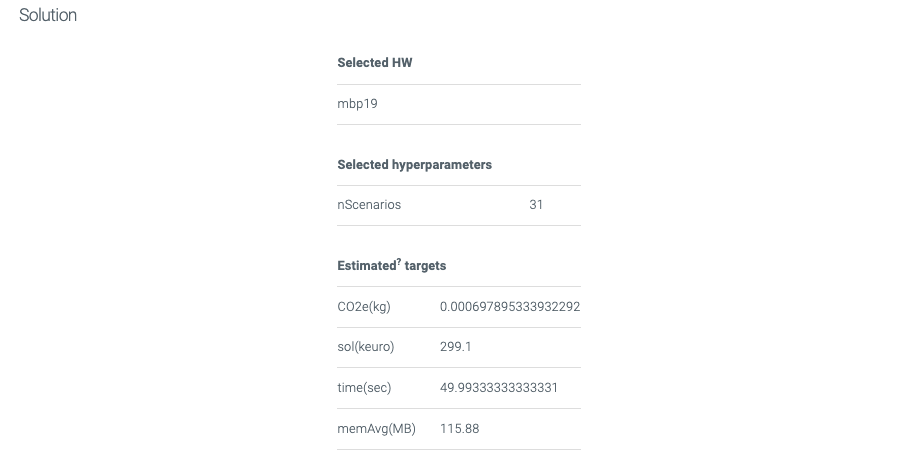
\includegraphics[width=\textwidth]{imgs/hada-solution-turkmenistan.png}
    \caption{Solution provided for the same constraint as in Figure~\ref{fig:hada_optimisation_req}, but this time selecting "Turkmenistan" as "Country"}
    \label{fig:hada_solution_turkmenistan}
\end{figure}

Comparing this to Figure~\ref{fig:hada_solution}, where Italy was the selected country, we observe a significant increase in CO₂ emissions:

\begin{itemize}
    \item Italy: $\approx 1.77 \times 10^{-4}$ kg CO$_2$e
    \item Turkmenistan: $\approx 6.98 \times 10^{-4}$ kg CO$_2$e
\end{itemize}

This increase highlights the critical role of geographic selection when running large-scale computations. While the absolute difference in emissions for a single execution might seem 
small, the impact becomes substantial when considering large workloads and multiple executions. This reinforces the importance of choosing greener energy grids whenever possible.

\subsection{Integration of Benchmark Data into HADA}

To expand HADA with additional benchmark data, datasets must be structured and formatted correctly. The standard organization for datasets is shown in Figure~\ref{fig:datasets_organization}.

\begin{figure}[h!]
    \centering
    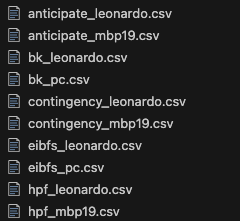
\includegraphics[width=0.8\linewidth]{imgs/benchmark-datasets.png}
    \caption{Organization of benchmark datasets for integration into HADA.}
    \label{fig:datasets_organization}
\end{figure}

\subsubsection{Dataset Format}

HADA expects datasets in \texttt{.csv} format, with files organized by \textbf{algorithm} and \textbf{platform}. Each dataset contains:
\begin{itemize}
    \item Algorithm Name
    \item Hardware Platform
    \item Hyperparameters (e.g., number of scenarios for ANTICIPATE)
    \item Target Performance Metrics (e.g., execution time, energy consumption, CO$_2$ emissions)
    \item Optional Input Parameters for input-dependent algorithms
\end{itemize}

\subsubsection{Metadata JSON Configuration}

In addition to dataset files, HADA requires a \textbf{JSON configuration file} specifying:
\begin{itemize}
    \item Algorithm details
    \item Hardware platform information
    \item Hyperparameter definitions
    \item Target performance metrics
    \item Constraints (if any)
\end{itemize}

Below is an example JSON structure:

\begin{verbatim}
{
    "name": "anticipate",
    "HW_ID": "macbook",
    "hyperparams": [
        {"ID": "num_scenarios", "type": "int", "LB": 1, "UB": 100}
    ],
    "targets": [
        {"ID": "time", "LB": null, "UB": null},
        {"ID": "memory", "LB": null, "UB": null},
        {"ID": "emissions", "LB": null, "UB": null}
    ]
}
\end{verbatim}

This approach allows HADA to seamlessly integrate new datasets, expanding its optimization capabilities to additional algorithms and hardware platforms. So, when data about the carbon
emissions or energy consumption of an algoritm, executed on different hardware platforms with different configurations, are available, they can be integrated in HADA. This could be 
very useful for choosing the optimal hardware architecture and algoritm configuration to minimize carbon emissions.

\chapter{Conclusions}

This research encountered several challenges, both technical and logistical, throughout its development. One of the primary obstacles was executing the ANTICIPATE and CONTINGENCY 
algorithms on the Leonardo HPC infrastructure. These algorithms rely on the Gurobi solver, which requires a valid license. However, due to system constraints, it was not possible to 
install the license directly on the compute nodes. To overcome this issue, it was necessary to coordinate with Gurobi's support team to obtain a Floating Academic License, which was 
subsequently installed on the CINECA License Server. This additional step introduced delays but ultimately enabled the successful execution of the algorithms on Leonardo.

Another significant challenge arose during the benchmarking phase of the Min-Cut/Max-Flow algorithms. The process involved managing a vast number of problem instances, many of which 
were extremely large, often reaching several gigabytes in size. Conducting experiments on multiple platforms required careful data management, computational resource allocation, and 
execution scheduling to ensure consistency across different architectures. Furthermore, systematically collecting, processing, and organizing the results into a structured dataset 
proved to be a highly time-consuming task. The need to execute these experiments on two distinct hardware platforms (Leonardo HPC and a personal workstation) added complexity, 
requiring careful tracking of execution conditions, runtime behavior, and performance variations.

Despite these challenges, this work successfully extended the HADA framework by integrating energy consumption and carbon footprint metrics using CodeCarbon. The experimental analysis 
provided valuable insights into the impact of hardware selection on computational efficiency, revealing that smaller-scale architectures (such as personal computers and laptops) tend
to be more energy-efficient for many of the tested workloads. However, the results also highlighted cases where HPC architectures like Leonardo could be preferable, particularly for 
large-scale problem instances, which exceeds the memory capacity of common devices. Moreover, the benchmark phase on Min-Cut/Max-Flow problems showed that the algorithms tested are 
very well optimized, so that they can achieve pretty good performances also on common devices, and this highligts the importance of efficient algorithm development for sustainability.
Additionally, this research underscores the importance of energy-aware computing and highlights how hardware selection, algorithm design, and execution environment can significantly 
influence the carbon footprint of computational tasks. The findings reinforce the potential for machine learning-driven optimization frameworks like HADA to assist in making informed 
decisions regarding computational resource usage, balancing trade-offs between runtime, memory consumption, energy efficiency, and emissions. Future work could explore further enhancements, such as integrating parallel Min-Cut/Max-Flow algorithms that could better leverage HPC architectures, refining the machine learning 
models used by HADA, or incorporating real-time carbon intensity data to dynamically optimize execution strategies based on current energy conditions. Expanding the benchmark dataset 
with additional algorithms and hardware configurations could further improve the accuracy and generalizability of HADA's optimization capabilities.
By addressing these challenges and proposing potential solutions, this study contributes to the broader effort of making computational research more sustainable, efficient, and 
environmentally conscious.

\appendix

\printbibliography[heading=bibintoc] % biblatex

\acknowledgements  
I would like to express my deepest gratitude to my supervisors, Andrea Borghesi and Allegra De Filippo, for their invaluable guidance, support, and encouragement throughout 
the development of this work. Their insights and expertise have been instrumental in shaping this research, and their contributions to the HADA framework provided the foundation 
upon which this study was built.  

I am also profoundly grateful to my family and friends for their unwavering support, patience, and encouragement throughout this long journey. Their belief in me has been a 
constant source of motivation, and this achievement would not have been possible without them.  

\end{document}